\documentclass[11pt,a4paper]{ctexart}
% Shared preamble for the assignment reports. Use with:
%   \documentclass[11pt,a4paper]{ctexart}  (XeLaTeX)
%   % Shared preamble for the assignment reports. Use with:
%   \documentclass[11pt,a4paper]{ctexart}  (XeLaTeX)
%   % Shared preamble for the assignment reports. Use with:
%   \documentclass[11pt,a4paper]{ctexart}  (XeLaTeX)
%   \input{../common/preamble.tex}
\usepackage[margin=2.3cm]{geometry}
\setmainfont{texgyretermes}[Extension=.otf,UprightFont=*-regular,BoldFont=*-bold,ItalicFont=*-italic,BoldItalicFont=*-bolditalic]
\setsansfont{texgyreheros}[Extension=.otf,UprightFont=*-regular,BoldFont=*-bold,ItalicFont=*-italic,BoldItalicFont=*-bolditalic]
\setmonofont{texgyrecursor}[Extension=.otf,UprightFont=*-regular,BoldFont=*-bold,ItalicFont=*-italic,BoldItalicFont=*-bolditalic]
\usepackage{amsmath,amssymb,mathtools,bm}
\usepackage{graphicx}
\usepackage{booktabs,multirow,makecell,array,tabularx}
\usepackage[table]{xcolor}
\usepackage[most]{tcolorbox}
\usepackage{enumitem}
\usepackage{listings}
\usepackage{subcaption}
\usepackage{siunitx}
\usepackage[hidelinks]{hyperref}
\usepackage[nameinlink,noabbrev]{cleveref}
\usepackage{float}

\setlength{\emergencystretch}{3em}
\linespread{1.15}
\setlist{leftmargin=*,itemsep=2pt,topsep=3pt}
\graphicspath{{figures/}}

\crefname{figure}{图}{图}
\crefname{table}{表}{表}
\crefname{section}{第}{第}
\creflabelformat{section}{#2#1#3 节}
\crefname{equation}{式}{式}
\crefformat{equation}{式~(#2#1#3)}

\lstset{basicstyle=\ttfamily\footnotesize,columns=fullflexible,breaklines=true,frame=single,
  framerule=0.3pt,rulecolor=\color{black!40},backgroundcolor=\color{black!3},
  keywordstyle=\color{blue!60!black}\bfseries,commentstyle=\color{green!40!black},
  numbers=left,numberstyle=\tiny\color{black!50},xleftmargin=1.5em}

% Interview boxes: question, model answer, common wrong answer.
\newtcolorbox{iqbox}[1]{enhanced,breakable,colback=blue!3,colframe=blue!45!black,boxrule=0.5pt,arc=1.5pt,
  left=4pt,right=4pt,top=3pt,bottom=3pt,fonttitle=\bfseries\small,title={面试追问：#1}}
\newtcolorbox{findingbox}[1][]{enhanced,breakable,colback=green!3,colframe=green!40!black,boxrule=0.5pt,arc=1.5pt,
  left=4pt,right=4pt,top=3pt,bottom=3pt,fonttitle=\bfseries\small,title={结论#1}}
\newtcolorbox{caveatbox}{enhanced,breakable,colback=orange!4,colframe=orange!60!black,boxrule=0.5pt,arc=1.5pt,
  left=4pt,right=4pt,top=3pt,bottom=3pt,fonttitle=\bfseries\small,title={不能推出的结论}}

\newcommand{\authorline}{ShaneLiu04\thanks{GitHub: \url{https://github.com/ShaneLiu04}。代码与原始指标：\url{https://gitee.com/liu-xingyan04/mlsys-infra}。本文基于公开课程材料独立完成，与课程团队无隶属关系。}}

\usepackage[margin=2.3cm]{geometry}
\setmainfont{texgyretermes}[Extension=.otf,UprightFont=*-regular,BoldFont=*-bold,ItalicFont=*-italic,BoldItalicFont=*-bolditalic]
\setsansfont{texgyreheros}[Extension=.otf,UprightFont=*-regular,BoldFont=*-bold,ItalicFont=*-italic,BoldItalicFont=*-bolditalic]
\setmonofont{texgyrecursor}[Extension=.otf,UprightFont=*-regular,BoldFont=*-bold,ItalicFont=*-italic,BoldItalicFont=*-bolditalic]
\usepackage{amsmath,amssymb,mathtools,bm}
\usepackage{graphicx}
\usepackage{booktabs,multirow,makecell,array,tabularx}
\usepackage[table]{xcolor}
\usepackage[most]{tcolorbox}
\usepackage{enumitem}
\usepackage{listings}
\usepackage{subcaption}
\usepackage{siunitx}
\usepackage[hidelinks]{hyperref}
\usepackage[nameinlink,noabbrev]{cleveref}
\usepackage{float}

\setlength{\emergencystretch}{3em}
\linespread{1.15}
\setlist{leftmargin=*,itemsep=2pt,topsep=3pt}
\graphicspath{{figures/}}

\crefname{figure}{图}{图}
\crefname{table}{表}{表}
\crefname{section}{第}{第}
\creflabelformat{section}{#2#1#3 节}
\crefname{equation}{式}{式}
\crefformat{equation}{式~(#2#1#3)}

\lstset{basicstyle=\ttfamily\footnotesize,columns=fullflexible,breaklines=true,frame=single,
  framerule=0.3pt,rulecolor=\color{black!40},backgroundcolor=\color{black!3},
  keywordstyle=\color{blue!60!black}\bfseries,commentstyle=\color{green!40!black},
  numbers=left,numberstyle=\tiny\color{black!50},xleftmargin=1.5em}

% Interview boxes: question, model answer, common wrong answer.
\newtcolorbox{iqbox}[1]{enhanced,breakable,colback=blue!3,colframe=blue!45!black,boxrule=0.5pt,arc=1.5pt,
  left=4pt,right=4pt,top=3pt,bottom=3pt,fonttitle=\bfseries\small,title={面试追问：#1}}
\newtcolorbox{findingbox}[1][]{enhanced,breakable,colback=green!3,colframe=green!40!black,boxrule=0.5pt,arc=1.5pt,
  left=4pt,right=4pt,top=3pt,bottom=3pt,fonttitle=\bfseries\small,title={结论#1}}
\newtcolorbox{caveatbox}{enhanced,breakable,colback=orange!4,colframe=orange!60!black,boxrule=0.5pt,arc=1.5pt,
  left=4pt,right=4pt,top=3pt,bottom=3pt,fonttitle=\bfseries\small,title={不能推出的结论}}

\newcommand{\authorline}{ShaneLiu04\thanks{GitHub: \url{https://github.com/ShaneLiu04}。代码与原始指标：\url{https://gitee.com/liu-xingyan04/mlsys-infra}。本文基于公开课程材料独立完成，与课程团队无隶属关系。}}

\usepackage[margin=2.3cm]{geometry}
\setmainfont{texgyretermes}[Extension=.otf,UprightFont=*-regular,BoldFont=*-bold,ItalicFont=*-italic,BoldItalicFont=*-bolditalic]
\setsansfont{texgyreheros}[Extension=.otf,UprightFont=*-regular,BoldFont=*-bold,ItalicFont=*-italic,BoldItalicFont=*-bolditalic]
\setmonofont{texgyrecursor}[Extension=.otf,UprightFont=*-regular,BoldFont=*-bold,ItalicFont=*-italic,BoldItalicFont=*-bolditalic]
\usepackage{amsmath,amssymb,mathtools,bm}
\usepackage{graphicx}
\usepackage{booktabs,multirow,makecell,array,tabularx}
\usepackage[table]{xcolor}
\usepackage[most]{tcolorbox}
\usepackage{enumitem}
\usepackage{listings}
\usepackage{subcaption}
\usepackage{siunitx}
\usepackage[hidelinks]{hyperref}
\usepackage[nameinlink,noabbrev]{cleveref}
\usepackage{float}

\setlength{\emergencystretch}{3em}
\linespread{1.15}
\setlist{leftmargin=*,itemsep=2pt,topsep=3pt}
\graphicspath{{figures/}}

\crefname{figure}{图}{图}
\crefname{table}{表}{表}
\crefname{section}{第}{第}
\creflabelformat{section}{#2#1#3 节}
\crefname{equation}{式}{式}
\crefformat{equation}{式~(#2#1#3)}

\lstset{basicstyle=\ttfamily\footnotesize,columns=fullflexible,breaklines=true,frame=single,
  framerule=0.3pt,rulecolor=\color{black!40},backgroundcolor=\color{black!3},
  keywordstyle=\color{blue!60!black}\bfseries,commentstyle=\color{green!40!black},
  numbers=left,numberstyle=\tiny\color{black!50},xleftmargin=1.5em}

% Interview boxes: question, model answer, common wrong answer.
\newtcolorbox{iqbox}[1]{enhanced,breakable,colback=blue!3,colframe=blue!45!black,boxrule=0.5pt,arc=1.5pt,
  left=4pt,right=4pt,top=3pt,bottom=3pt,fonttitle=\bfseries\small,title={面试追问：#1}}
\newtcolorbox{findingbox}[1][]{enhanced,breakable,colback=green!3,colframe=green!40!black,boxrule=0.5pt,arc=1.5pt,
  left=4pt,right=4pt,top=3pt,bottom=3pt,fonttitle=\bfseries\small,title={结论#1}}
\newtcolorbox{caveatbox}{enhanced,breakable,colback=orange!4,colframe=orange!60!black,boxrule=0.5pt,arc=1.5pt,
  left=4pt,right=4pt,top=3pt,bottom=3pt,fonttitle=\bfseries\small,title={不能推出的结论}}

\newcommand{\authorline}{ShaneLiu04\thanks{GitHub: \url{https://github.com/ShaneLiu04}。代码与原始指标：\url{https://gitee.com/liu-xingyan04/mlsys-infra}。本文基于公开课程材料独立完成，与课程团队无隶属关系。}}

\graphicspath{{../../solutions/cmu15849/compiler-compression/artifacts/figures/}}
\usepackage{adjustbox}

\title{CMU 15-849 编译与压缩：从 CPU 代价模型到 RTX 5090 实测\\\large 算子融合、调度搜索、量化、剪枝与 LoRA 的论文复现}
\author{\authorline}
\date{2026 年 10 月}

\begin{document}
\maketitle

\begin{abstract}
本文是 CMU 15-849（Machine Learning Systems）编译与压缩专题的复现报告。这门课是论文研讨课，没有编程作业，
所以我们把 TVM、Ansor、TASO、XLA、PyTorch~2（TorchInductor）、Triton、LLM.int8、SmoothQuant、GPTQ、AWQ、LoRA、QLoRA 与 Deep Compression 的核心算法各做成一个可测试的最小实现。
每个问题都分两步回答：先在 CPU 上建立\emph{模型}（反向模式自动微分、带融合 pass 的图 IR、带代价模型的调度搜索，以及量化、剪枝、LoRA 的数值实验，共 29 个 CPU 测试），
再到 RTX~5090（sm\_120）上做\emph{测量}，看模型说对了多少。

主要发现有五条。
(1) 在访存受限的算子链上，\texttt{torch.compile} 的加速比几乎就等于“eager 字节 / 融合字节”，两者相差不到 7\%（RMSNorm 实测 9.86$\times$，字节比 10.0$\times$），融合后的 kernel 稳定在 1.41--1.61 TB/s。
含 GEMM 的 MLP 只快 15\%，实验室图 IR 的 roofline 预测落在实测的 4--6\% 以内。max-autotune 打开的 CUDA graph 要先拷贝输入，让大张量上的访存受限 kernel 慢了 2.08$\times$。
(2) 一个 30 行的 Triton matmul 在 $8192^3$ 上达到 221.5 TFLOP/s（cuBLAS 为 214.3），但最优 tile 随形状变化；两个解析代价模型的排序相关（Spearman $\rho$）在 0.10--0.72 之间，各自只抓住了一种效应。
(3) GPT-2 上 int8 per-channel 量化无损；到 int3 g128 时，GPTQ 把困惑度从 65.92 拉回 37.24。SmoothQuant 的 $\alpha$ 选错（0.5），per-tensor W8A8 会崩到 407。
速度上，int8 GEMM 是 bf16 的 3.0$\times$（679 vs 227 TOP/s）；batch 1 时 W8 和 W4 的 GEMV 分别快 1.8--2.0$\times$ 和 2.3--2.7$\times$，原因只是读的字节少了。
(4) 一次性剪掉 50\% 权重，幅值剪枝的困惑度是 538，Wanda 只有 47；2:4 稀疏经 cuSPARSELt 在大 GEMM 上快 1.54--1.58$\times$，小 $M$ 时反而更慢。
(5) LoRA 把 GPT-2 medium 微调的峰值显存从 16.07 降到约 12.1 GiB，省下的正好是 AdamW 状态；$r{=}16$ 的验证损失 2.874 略好于全量微调的 2.891。
\end{abstract}

\tableofcontents
\newpage

\section{背景与作业要求}

编译器和模型压缩在课程里是两个单元，但它们面对的是同一类问题：模型的数学已经定了，怎样让它在 GPU 上少搬字节、少等硬件？
编译器的办法是把算子融合在一起、为每个算子挑一个好的分块方式；压缩的办法是用更少的位数表示权重，或者干脆去掉一部分权重。
这两类方法的论文里都有很漂亮的模型，而这份报告想知道的是：这些模型在一张真实的 GPU 上还能说对多少。

15-849 没有官方编程作业。我们把两个单元的必读论文整理成五个可以测量的问题。
每个问题都有一个 CPU 侧的\emph{模型}（此前已经实现）和一个 GPU 侧的\emph{测量}（本次新增），对应关系见下表。

\begin{table}[H]
\centering\small
\begin{tabularx}{\linewidth}{p{2.6cm}p{3.6cm}X}
\toprule
问题 & 论文 & CPU 侧模型 $\rightarrow$ GPU 侧测量 \\
\midrule
Q1 算子融合 & TVM~\cite{tvm}、XLA~\cite{xla}、TASO~\cite{taso}、PyTorch~2 / TorchInductor~\cite{pt2} & 图 IR 的逐元素/epilogue 融合 pass 与 roofline~\cite{roofline} 字节模型 $\rightarrow$ eager vs \texttt{torch.compile}（default / max-autotune）、手写 Triton~\cite{triton} 融合 kernel、编译时间与动态 shape 重编译 \\
Q2 调度搜索 & Halide~\cite{halide}、TVM、Ansor~\cite{ansor}、Triton & 单 SM 解析代价模型 + grid/random/进化搜索 $\rightarrow$ Triton matmul 的 192 点分块网格实测、autotune、cuBLAS、代价模型的 Spearman 排序相关 \\
Q3 量化 & LLM.int8~\cite{llmint8}、SmoothQuant~\cite{smoothquant}、GPTQ~\cite{gptq}、AWQ~\cite{awq} & 合成矩阵上的误差 $\rightarrow$ GPT-2~\cite{gpt2} 124M/355M 在 wikitext-2~\cite{wikitext} 上的困惑度；int8/FP8 GEMM 与 W8/W4 weight-only GEMV 吞吐 \\
Q4 剪枝 & Deep Compression~\cite{deepcomp}、NVIDIA 2:4~\cite{nm}、Wanda~\cite{wanda} & 合成矩阵与小 MLP $\rightarrow$ GPT-2 困惑度、cuSPARSELt 2:4 与 CSR 的 kernel 速度 \\
Q5 LoRA~\cite{lora} & LoRA、QLoRA~\cite{qlora} & 单层低秩拟合 $\rightarrow$ GPT-2 medium 全量微调 vs LoRA $r{=}4..64$ vs int8/int4 冻结基座，显存/步时/损失曲线/合并等价 \\
\bottomrule
\end{tabularx}
\caption{每个问题对应的论文，以及它在 CPU 侧的模型和 GPU 侧的测量。}
\end{table}

文中每个数字都能追溯到原始记录：CPU 结果在 \texttt{artifacts/raw/*.csv}，GPU 结果在 \texttt{artifacts/raw/gpu/*.jsonl}。
加速比、Spearman 相关、实验室模型在 RTX 5090 参数下的预测这类派生量，由 \texttt{scripts/plot\_gpu.py} 统一算出，写入 \path{artifacts/raw/gpu/summary_gpu.json}。

\section{实验环境}

GPU 结果都在一张 RTX 5090 上测得。下表里有两项会在后文反复出现：96 MB 的 L2 决定了多大的张量才能测出真实的显存带宽，
每 block 99 KB 的共享内存上限决定了哪些 Triton 配置根本跑不起来。

\begin{table}[H]
\centering\small
\begin{adjustbox}{max width=\linewidth}\begin{tabular}{ll}
\toprule
CPU 侧 & Windows Server，4 物理核 / 8 逻辑核；Python 3.12，numpy、torch CPU、pytest \\
GPU & NVIDIA GeForce RTX 5090（Blackwell，sm\_120），170 SM，32 GB GDDR7，96 MB L2，驱动 595.71.05 \\
GPU 峰值（规格） & bf16 稠密（fp32 累加）209.5 TFLOP/s；显存带宽 1.792 TB/s（实测 saxpy 约 1.55 TB/s） \\
共享内存 & 每 block 上限 101376 B（99 KB，Triton/Inductor 报错信息中给出） \\
软件 & PyTorch 2.8.0+cu128，Triton 3.4.0，CUDA 12.8，transformers 5.21.0 \\
服务器 CPU & 仅用 2 个核（\texttt{taskset -c 47,48}，\texttt{OMP\_NUM\_THREADS=2}，Inductor 编译线程 2） \\
GPU 互斥 & 所有 GPU 命令经 \texttt{flock /root/autodl-tmp/gpu.lock}，计时不受其他实验干扰 \\
\bottomrule
\end{tabular}\end{adjustbox}
\caption{实验环境。\texttt{tools/mlsys\_calc.py} 里没有收录 RTX 5090，所以我们在 \texttt{gpu/common.py} 中按同样的字段（bf16 峰值、带宽）定义它，再用 \texttt{mlsys\_calc.GPU} 构造对象，交给实验室的代价模型。}
\end{table}

计时用 CUDA event 包住 $n$ 次调用。$n$ 自动选取，使一组耗时约 20--50 ms；先预热 $n/5$ 次，再取 5 组的中位数。
编译相关的实验设置了 \texttt{TORCHINDUCTOR\_FORCE\_DISABLE\_CACHES=1}，并且每次使用全新的 \texttt{TRITON\_CACHE\_DIR}，所以首次调用的时间就是真实的冷编译成本。
kernel 数用 \texttt{torch.profiler}（CUDA activity）统计：数 5 次调用中的 kernel 事件（不含 memcpy/memset），再取平均。

\section{方法与实现}

\subsection{代码结构}

CPU 侧的算法都在 \texttt{code/compkit/} 里；GPU 侧每个问题一个脚本，画图和汇总在本地完成，不占 GPU。

\begin{lstlisting}[language={}]
compiler-compression/
  code/compkit/      autodiff, graph_ir (fusion/CSE/TASO merge), schedule_search, quantization, pruning, lora
  gpu/common.py      CUDA-event timing, JSONL writer, RTX 5090 numbers
  gpu/triton_kernels.py  fused RMSNorm, fused bias+GELU, tiled matmul (+autotune), W8A16/W4A16 GEMV
  gpu/fusion_bench.py    Q1: chains / mlp / triton / dynamic
  gpu/matmul_search.py   Q2: 192-config tile grid vs autotune vs cuBLAS
  gpu/llm_utils.py, quant_llm.py, quant_speed.py   Q3: PTQ on GPT-2, low-precision GEMM/GEMV
  gpu/prune_bench.py     Q4: one-shot pruning ppl, 2:4 cuSPARSELt and CSR speed
  gpu/lora_ft.py         Q5: full FT vs LoRA vs QLoRA-like
  gpu/run_gpu.sh         runner (each step under flock, taskset)
  scripts/plot_gpu.py    all GPU figures + summary_gpu.json (local, no GPU)
  tests/test_gpu.py      11 tests: 7 CPU-runnable algorithm tests, 4 CUDA kernel tests (skip w/o CUDA)
\end{lstlisting}

\subsection{Q1：eager 字节计数器与融合基准}

要检验“融合省掉多少字节就快多少”，先得知道 eager 模式到底搬了多少字节。我们用 \texttt{TorchDispatchMode}（PyTorch 提供的钩子，能拦截每一次 aten 算子调用）
把每个非视图算子的输入与输出张量字节数加起来。这和实验室图 IR 里 \texttt{kernel\_cost} 的假设完全相同：每个 kernel 把输入读一次、把输出写一次，不考虑 L2 复用。
区别只在于，这里统计的是真实的 PyTorch 程序：

\begin{lstlisting}[language=Python]
class ByteCounter(TorchDispatchMode):
    def __torch_dispatch__(self, func, types, args=(), kwargs=None):
        out = func(*args, **(kwargs or {}))
        if func.overloadpacket.__name__ not in _VIEW_OPS:
            for t in unique_tensors(args, kwargs, out):
                self.bytes += t.numel() * t.element_size()
        return out
\end{lstlisting}

与之对照的“融合理想字节”是整条链的下界：图输入读一次、图输出写一次，权重也计入。我们把“达到带宽”定义为理想字节除以实测时间。
这个定义有一个副作用：理想字节小于 96 MB 的 L2 时，反复计时同一份输入会命中 L2，算出的“带宽”可以超过 GDDR7 峰值。
这不是计时错误，后面的带宽图会用黄色区域把这部分标出来。

我们还手写了一个 Triton RMSNorm 作参照。每个 program 处理一行，整行一次装进寄存器，归约用 fp32：
\begin{lstlisting}[language=Python]
@triton.jit
def _rmsnorm_kernel(x_ptr, w_ptr, y_ptr, n_cols, eps, BLOCK: tl.constexpr):
    row = tl.program_id(0)
    cols = tl.arange(0, BLOCK); mask = cols < n_cols
    x = tl.load(x_ptr + row * n_cols + cols, mask=mask, other=0.0).to(tl.float32)
    w = tl.load(w_ptr + cols, mask=mask, other=0.0).to(tl.float32)
    rstd = tl.rsqrt(tl.sum(x * x, axis=0) / n_cols + eps)
    tl.store(y_ptr + row * n_cols + cols, (x * rstd * w).to(y_ptr.dtype.element_ty), mask=mask)
\end{lstlisting}

\subsection{Q2：Triton matmul 网格与代价模型}

\texttt{\_matmul\_kernel} 是标准的分块 matmul，带 grouped ordering（按组排列 program，让相邻 program 共享 A 的行块，提高 L2 命中）。
每个 program 负责一个 $B_M\times B_N$ 的 C 块，沿 K 方向每次前进 $B_K$，用 \texttt{tl.dot} 累加到 fp32。
我们扫描的网格是 $B_M,B_N\in\{32,64,128,256\}$、$B_K\in\{32,64\}$、\texttt{num\_warps}$\in\{4,8\}$、\texttt{num\_stages}$\in\{2,3,4\}$，共 192 个点。
共享内存超过 99 KB 的配置无法运行，记为 OOR（out of resource）。
对照组有两个：同一个 kernel 加上 \texttt{@triton.autotune}（使用 Triton 教程里的 10 个候选），以及 cuBLAS（直接写 \texttt{A @ B}）。

然后我们问：不跑 kernel，光靠解析模型能不能把这些配置排对？两个代价模型各自给 $(B_M,B_N,B_K)$ 三元组排序；
实测一侧取该三元组在所有 warps/stages 组合上的最好值，再计算两者的 Spearman $\rho$（排序相关系数，1 表示完全排对）。
\begin{enumerate}
\item 实验室模型：\texttt{schedule\_search.cost(Schedule("ijk", BM, BN, BK))}，参数换成 RTX 5090 每个 SM 的份额（$209.5/170$ TFLOP/s、$1.792/170$ TB/s、99 KB 缓存）。Triton 的一个 program 恰好对应“ij 在外层、k 在内层”的循环序。
\item 波次量化 roofline：$T = \lceil \#\text{tiles}/170\rceil\cdot\max\bigl(\frac{2B_MB_NK}{P/170},\frac{2(B_M+B_N)K}{BW/170}\bigr)$。它比普通 roofline 只多考虑了一件事：C 块在 170 个 SM 上是一波一波执行的。
\end{enumerate}

\subsection{Q3：GPT-2 上的 PTQ}

PTQ（post-training quantization，训练后量化）只用少量校准数据，不再训练。我们量化 GPT-2 每个 block 内的全部线性层，
即 \texttt{c\_attn}、\texttt{attn.c\_proj}、\texttt{c\_fc}、\texttt{mlp.c\_proj}，124M 模型共 48 个；嵌入与共享权重的 \texttt{lm\_head} 保持 fp16。
困惑度在完整的 wikitext-2 test 上计算：287,644 个 token，按 1024 切成 280 个不重叠窗口。校准集是从 train 中随机取的 128 个 1024-token 窗口。

GPTQ 是我们自己实现的，按 block 顺序进行。处理第 $l$ 个 block 时，先用前 $l-1$ 个 block 已经量化的模型做前向，得到该 block 线性层的输入统计 $H=\frac1n\sum xx^\top$（即层输出误差关于权重的 Hessian）。
然后对这个 block 的四个线性层分别做列序 OBQ~\cite{obq} 更新：每量化一列，就把误差按 $H^{-1}$ 推给还没量化的列。
实现上每 128 列做一次 lazy batch 更新，阻尼取平均对角元的 1\%：
\begin{lstlisting}[language=Python]
Hinv = torch.linalg.cholesky(torch.cholesky_inverse(torch.linalg.cholesky(H)), upper=True)
for i1 in range(0, cols, block):
    W1, Hi = W[:, i1:i2].clone(), Hinv[i1:i2, i1:i2]
    for i in range(i2 - i1):
        if (i1 + i) % g == 0: s, z = asym_params(W1[:, i:i + g], bits)  # group grid
        q = asym_q(W1[:, i:i+1], s, z, bits)
        err = (W1[:, i:i+1] - q) / Hi[i, i]
        W1[:, i:] -= err @ Hi[i:i+1, i:]          # push error onto unquantized columns
        Q1[:, i:i+1], E1[:, i:i+1] = q, err
    W[:, i2:] -= E1 @ Hinv[i1:i2, i2:]            # lazy update of later blocks
\end{lstlisting}

AWQ 风格的方法按激活幅度缩放输入通道：$s_j=\overline{|x_j|}^{a}$，在 $a\in\{0,0.1,\dots,1\}$ 上网格搜索，用代理误差 $\operatorname{tr}(\Delta W H\Delta W^\top)$ 选出最优的 $a$，这里复用 GPTQ 的同一个 $H$。

W8A8 同时量化权重和激活，我们只做模拟。权重一律 per-channel int8；激活用 per-tensor 或 per-token 的动态 absmax int8。
SmoothQuant 用校准集上的 $\max|X_j|$ 计算 $s_j=\max|X_j|^\alpha/\max|W_j|^{1-\alpha}$，把激活的尺度挪一部分给权重，$\alpha$ 取 0.5 与 0.8。
LLM.int8 动态找出任意 token 上 $|x|>6$ 的输入列，这些列用 fp16 计算，其余列走 per-token$\times$per-channel 的 int8。
所有 W8A8 方案都是“量化再反量化”，实际仍用 fp16 GEMM 计算，因此只评估精度，不评估速度。

速度单独测。int8 用 \texttt{torch.\_int\_mm}（int32 累加），结果与 fp64 参考逐元素比较；FP8 用 \texttt{torch.\_scaled\_mm}（e4m3，张量 scale=1）。
batch 1 的 weight-only 量化（只量化权重、激活仍是 bf16）用我们自写的 Triton GEMV：W8A16 每行一个 scale；W4A16 每字节存两个 int4，每 128 个元素一组 fp16 scale，在 kernel 内解包和反量化。
4096$\times$4096 这样的权重只有 32 MB，会常驻 96 MB 的 L2，测出来过于乐观。所以“cold”模式轮换多份权重副本，让工作集超过 384 MB。

\subsection{Q4/Q5：剪枝与 LoRA}

剪枝都是一次性的，剪完不再微调。我们比较了三类方法：幅值剪枝（每层一个全局阈值）的 30/50/70\% 稀疏度、幅值剪枝的 2:4 与 4:8 结构（每 4 个或 8 个元素里留一半），
以及 Wanda 的 50\% 与 2:4。Wanda 的打分是 $|W_{ij}|\cdot\|X_j\|_2$，在每个输出行内部比较。
速度方面测两种稀疏格式：\texttt{to\_sparse\_semi\_structured}（2:4，有 cuSPARSELt 与 CUTLASS 两个后端）和 \texttt{to\_sparse\_csr}（非结构化）。

LoRA 实验用 GPT-2 medium（355M），在 wikitext-2 train 上训练 150 步，batch 为 8$\times$512，使用 bf16 autocast。
全量微调用 AdamW，lr $3\times10^{-5}$，保留 fp32 主权重。LoRA 挂在所有 block 内的线性层上，$\alpha=2r$，lr $10^{-3}$，基座以 bf16 冻结。
QLoRA-like 配置把冻结基座存成 int8（per-channel）或 int4（g128 打包），用一个自定义的 \texttt{autograd.Function} 在前向和反向里各反量化一次，并且\emph{只保存量化张量}。
这一点不能省：如果直接把反量化出的权重交给 \texttt{F.linear}，autograd 会把这份 bf16 权重存进计算图，显存一点也不会少。

\section{实验结果}

\subsection{Q0：CPU 侧基础——自动微分与图 pass 的正确性}

后面所有的字节模型都建立在一个前提上：图 pass 只改变 kernel 的边界，不改变计算结果。所以先确认这一点。
在两层 MLP 加 softmax 交叉熵上，自写反向模式自动微分的梯度与 torch 的最大差 $\le 5.6\times10^{-17}$，与中心差分的最大差 $\le 2.3\times10^{-10}$（\texttt{autodiff\_check.csv}）。
拓扑排序是迭代实现的，5000 层的链式乘法做反向也不会爆栈（有测试覆盖）。
图 IR 的常量折叠、CSE、逐元素融合和 epilogue 融合前后，解释器输出的最大差为 0；TASO 式 matmul 合并后为 $1.7\times10^{-18}$（\texttt{graph\_pass\_checks.csv}）。

\subsection{Q1：算子融合——字节模型 vs 实测}

同一个模型，打开 \texttt{torch.compile} 有时快十倍，有时几乎不变。这一节想说清楚原因：融合到底省了什么，以及能不能在跑之前就算出它能省多少。

\paragraph{CPU 模型（H100 参数）。}先看实验室图 IR 的预测。\Cref{fig:cpu-fusion} 是它在 $T{=}4096,d{=}4096,d_{ff}{=}16384$ 的 MLP 上的结果。
不融合时有 7 个 kernel，HBM 流量 1.376 GB。逐元素融合后剩 5 个 kernel、1.040 GB（$-24\%$）；再把逐元素算子并进 GEMM 的 epilogue（GEMM 写回结果前顺手做的尾部计算），剩 3 个、0.705 GB（$-49\%$）。
流量减了一半，roofline 时间却只从 1342 µs 降到 1132 µs（$-16\%$），因为两个 GEMM 各要 556 µs，而且是计算受限的，融合碰不到它们。
由此得到一个可以检验的预测：\emph{融合对访存受限链收益巨大，对含大 GEMM 的块收益很小}。

\begin{figure}[H]
\centering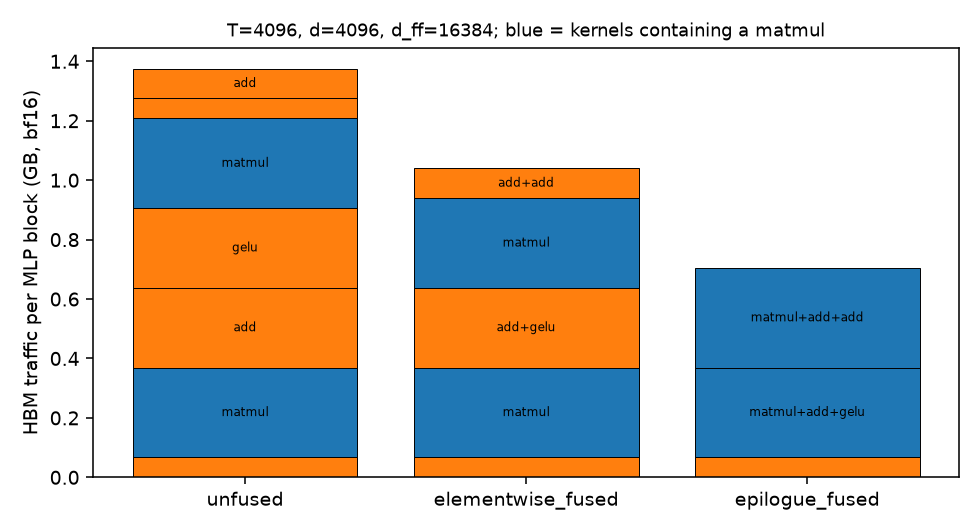
\includegraphics[width=0.75\linewidth]{fusion_traffic.png}
\caption{（CPU 模型）实验室图 IR 的融合 pass 对 Transformer MLP 的 HBM 流量与 roofline 时间的预测。流量和时间下降的幅度差得很远。}
\label{fig:cpu-fusion}
\end{figure}

\paragraph{GPU 实测：访存受限链。}先检验预测里“收益巨大”的那一半。我们选了五条常见的访存受限链，在 $M\in\{256,1024,4096,16384\}$、$N{=}4096$、bf16 下比较 eager 与 Inductor，
结果见 \cref{fig:fusion-speedup,fig:fusion-bw,fig:fusion-kb}。\Cref{tab:fusion} 只列最大尺寸：这时每个张量 128 MB，超出了 L2，测到的才是真正的显存带宽。

\begin{table}[H]
\centering\small
\begin{adjustbox}{max width=\linewidth}\begin{tabular}{lrrrrrr}
\toprule
链 & eager kernel 数 & eager µs & Inductor µs & 实测加速 & 字节比（eager/理想） & Inductor TB/s \\
\midrule
RMSNorm（fp32 手写式） & 9 & 1723.8 & 174.9 & 9.86$\times$ & 10.0$\times$ & 1.54 \\
softmax（fp32 上转） & 3 & 885.4 & 175.3 & 5.05$\times$ & 5.0$\times$ & 1.53 \\
bias+GELU+dropout & 3 & 580.3 & 190.1 & 3.05$\times$ & 3.25$\times$ & 1.41 \\
残差链（4 输入） & 5 & 1116.7 & 417.2 & 2.68$\times$ & 2.60$\times$ & 1.61 \\
LayerNorm（\texttt{F.layer\_norm}） & 1 & 176.0 & 175.0 & 1.01$\times$ & 1.00$\times$ & 1.53 \\
\bottomrule
\end{tabular}\end{adjustbox}
\caption{$M{=}16384$ 时 eager 与 Inductor（default 模式）的对比。eager 字节由 dispatch 计数器得到，理想字节按“输入读一次、输出写一次”计算（\texttt{fusion\_chains.jsonl}）。}
\label{tab:fusion}
\end{table}

表里最该对比的是“实测加速”和“字节比”两列，它们几乎一样。

\begin{findingbox}[：字节比就是加速比]
在不命中 L2 的尺寸上，Inductor 相对 eager 的实测加速与“eager 字节 / 理想字节”相差不到 7\%；融合后的 kernel 都稳定在 1.41--1.61 TB/s，已经顶在带宽墙上。
\end{findingbox}

具体来说，RMSNorm 是 9.86$\times$ 对 10.0$\times$，softmax 是 5.05$\times$ 对 5.0$\times$，残差链是 2.68$\times$ 对 2.60$\times$。
1.41--1.61 TB/s 相当于 GDDR7 峰值的 79--90\%，或 saxpy 实测带宽的 91--104\%。
这正是实验室 \texttt{kernel\_cost} 的模型：访存受限算子的时间等于字节除以带宽，融合做的事只是删掉中间张量的一次写和一次读。
LayerNorm 是个有用的反例：\texttt{F.layer\_norm} 在 eager 下本来就是一个手写好的融合 kernel，Inductor 没有字节可省，所以只有 1.01$\times$。

表里只有最大尺寸。下面三张图把尺寸这一维展开，分别看加速比、带宽和 kernel 数怎样随 $M$ 变化。

\begin{figure}[H]
\centering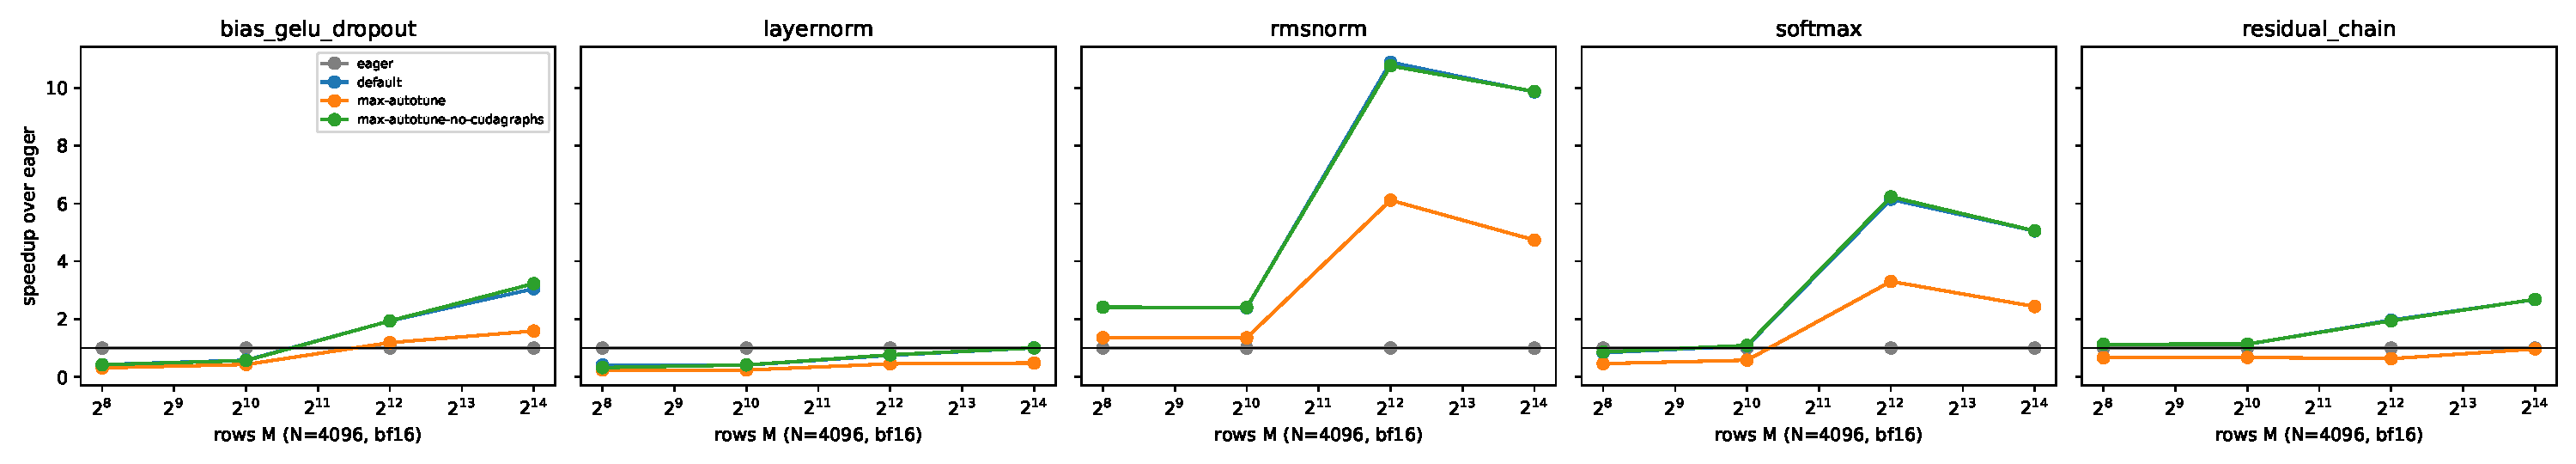
\includegraphics[width=\linewidth]{gpu_fusion_speedup.pdf}
\caption{各链相对 eager 的加速比随行数 $M$ 的变化（$N{=}4096$）。小尺寸下编译版本反而\emph{更慢}，因为这时 kernel 本身很短，固定开销占了大头：编译版本每次调用有约 23--27 µs 的 Python/guard 开销，而 eager 单个 kernel 约 11 µs；max-autotune 的 CUDA graph 还要先把输入拷进静态缓冲区。}
\label{fig:fusion-speedup}
\end{figure}

\begin{figure}[H]
\centering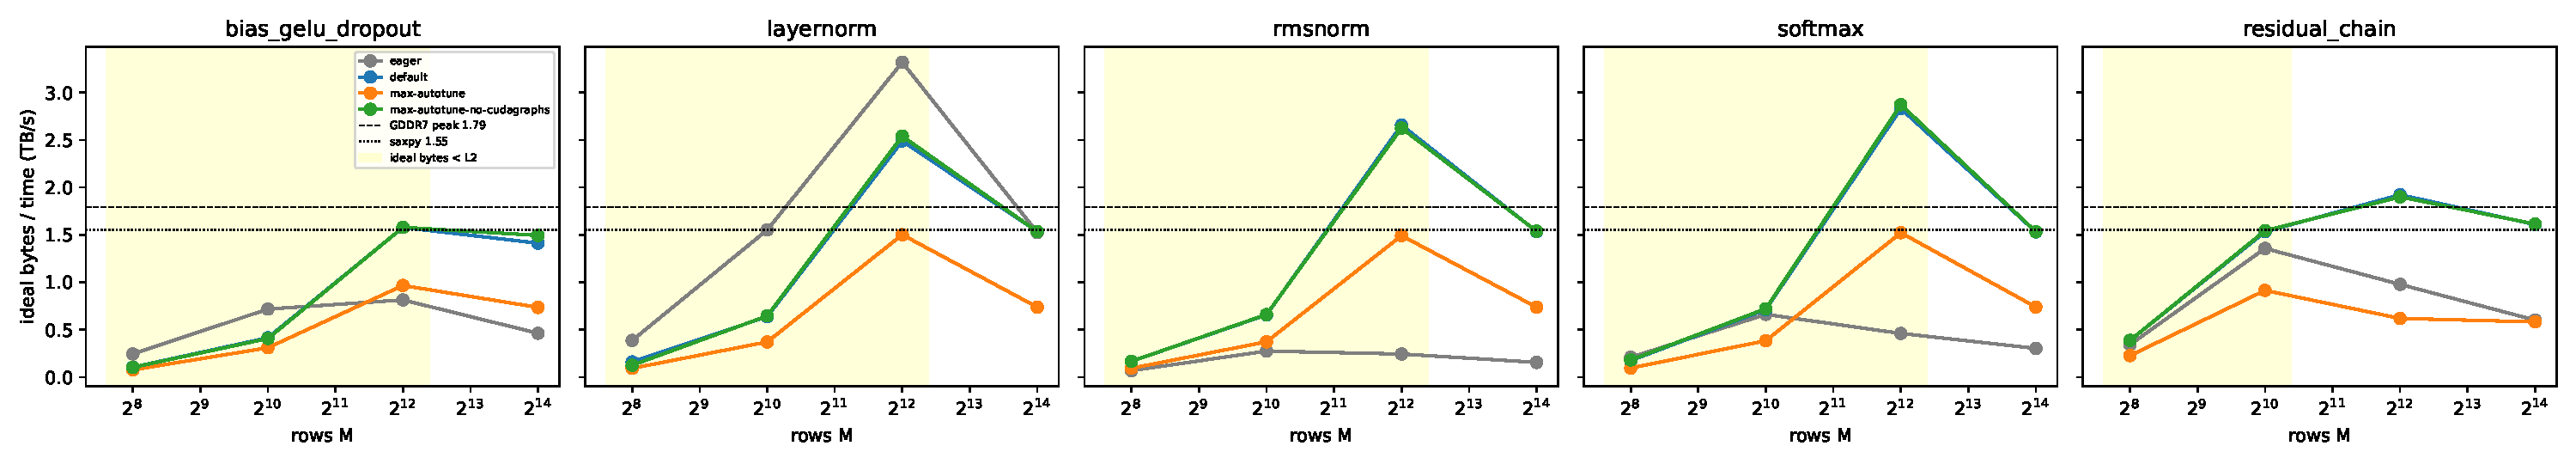
\includegraphics[width=\linewidth]{gpu_fusion_bandwidth.pdf}
\caption{达到带宽 = 理想字节 / 时间。黄色区域里理想字节小于 96 MB 的 L2，反复计时同一输入会命中 L2，所以“带宽”可以高于 GDDR7 峰值：LayerNorm 在 $M{=}4096$（67 MB）时 eager 达到 3.32 TB/s，RMSNorm/softmax 的 Inductor 版本达到 2.66/2.83 TB/s。到 $M{=}16384$，所有融合版本都回落到 1.53 TB/s 左右，这才是显存带宽。}
\label{fig:fusion-bw}
\end{figure}

\begin{figure}[H]
\centering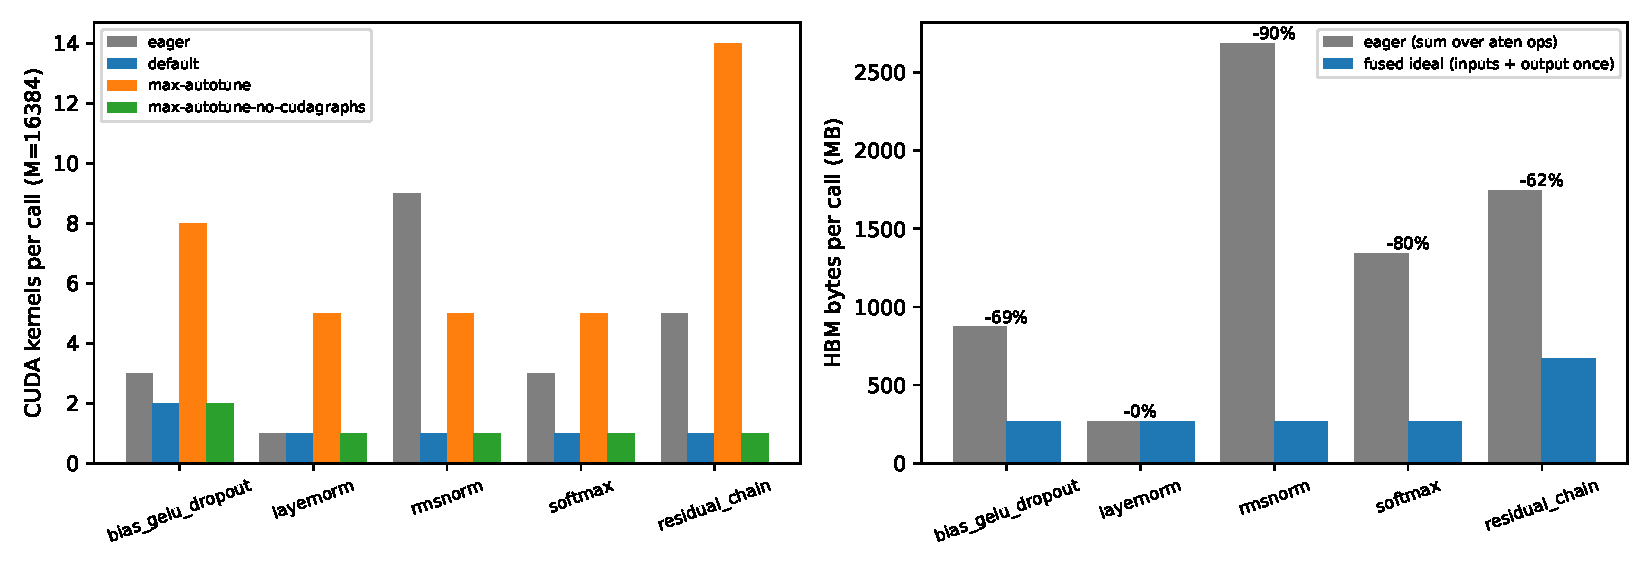
\includegraphics[width=\linewidth]{gpu_fusion_kernels_bytes.pdf}
\caption{左：$M{=}16384$ 时每次调用的 CUDA kernel 数。default 与 no-cudagraphs 都把每条链压成 1--2 个 kernel；max-autotune（开 CUDA graph）多出 3--13 个 kernel，它们是 cudagraph tree 把非静态输入拷进图内缓冲区的 copy kernel。右：eager 字节与融合理想字节，标出了省下的比例（RMSNorm 90\%、softmax 80\%、bias+GELU+dropout 69\%、残差链 62\%、LayerNorm 0\%）。省得越多的链，加速越大。}
\label{fig:fusion-kb}
\end{figure}

\paragraph{一个反直觉的结果：max-autotune 让访存受限链变慢 2$\times$。}左图里 max-autotune 多出来的 copy kernel 不是摆设。
$M{=}16384$ 时，max-autotune 下的 RMSNorm、softmax 和 LayerNorm 都要约 364 µs，default 只要约 175 µs；而 \texttt{max-autotune-no-cudagraphs} 与 default 相同（174.5 µs）。
所以区别只在 CUDA graph。CUDA graph 要求输入位于固定地址，而我们的输入张量不是，于是每次 replay 前都得先拷贝一遍。
对一个读 128 MB、写 128 MB 的 kernel，这次拷贝正好让流量翻倍。残差链有 4 个输入，max-autotune 下要 1152.7 µs，比 eager 的 1116.7 µs 还慢。
CUDA graph 省的是 launch 开销，每个 kernel 只有几 µs，只有在 kernel 很短、调用很密的场景（比如 decode）才划算；对大张量上的单个 kernel，它是负优化。

\paragraph{含 GEMM 的 MLP 与 Transformer block。}接下来检验预测的另一半：GEMM 占主导时，融合还能省多少？
我们测的 MLP 取 $d{=}1024$、$d_{ff}{=}4096$，结构与实验室的 \texttt{transformer\_mlp} 完全相同（LN、W1+b1、GELU、W2+b2、残差），结果见 \cref{tab:mlp} 与 \cref{fig:mlp}。
表的下半部分是实验室模型换上 RTX 5090 参数后的预测，可以直接和上半部分的实测比。

\begin{table}[H]
\centering\small
\begin{tabular}{lrrrrr}
\toprule
（$T{=}4096$） & kernel 数 & 时间 µs & TFLOP/s & 首调用/编译 s & 与 eager 最大差 \\
\midrule
eager & 5.0 & 419.4 & 163.9 & -- & 0 \\
Inductor default & 5.0 & 414.4 & 165.8 & 0.59 & 0.031 \\
Inductor max-autotune & 4.0 & 366.8 & 187.4 & 6.91 & 0.031 \\
max-autotune-no-cudagraphs & 2.8 & 356.8 & 192.6 & 6.45 & 0.031 \\
\midrule
实验室模型（5090 参数）不融合 & 7 & 435.7 & -- & -- & -- \\
实验室模型 逐元素融合 & 5 & 388.9 & -- & -- & -- \\
实验室模型 + epilogue & 3 & 338.1 & -- & -- & -- \\
\bottomrule
\end{tabular}
\caption{Transformer MLP，$T{=}4096$（\texttt{fusion\_mlp.jsonl}；模型行来自 \texttt{summary\_gpu.json} 中的 \texttt{lab\_mlp\_model\_5090}）。}
\label{tab:mlp}
\end{table}

\begin{findingbox}[：实验室模型对 MLP 的预测落在实测的 4\% 内]
实验室图 IR 预测不融合的 MLP 为 435.7 µs，eager 实测 419.4 µs（低 3.7\%）；预测全融合为 338.1 µs，max-autotune-no-cudagraphs 实测 356.8 µs（高 5.5\%）。
\end{findingbox}

模型和实测之间有一处结构上的差别：eager 只有 5 个 kernel，而不是模型里的 7 个，因为 cuBLASLt 的 \texttt{addmm} 本来就把 bias 融进了 GEMM 的 epilogue。
default 模式几乎没有收益（414.4 vs 419.4 µs，$-1.2\%$）。它只是重排了 GELU 等逐元素算子，GEMM 仍然调用 cuBLAS。
max-autotune 的 $-15\%$ 主要来自 Triton 的 GEMM 模板：它把 GELU 和残差做进 epilogue，还选到了更好的 tile。代价是编译时间从 0.59 s 涨到 6.91 s（11.7$\times$）。
含 SDPA 的完整 block 也是同样的规律：eager 712.4 µs，default 694.3 µs，max-autotune 621.6 µs，no-cudagraphs 607.0 µs（$-14.8\%$），编译要 12.2--12.9 s。

\begin{figure}[H]
\centering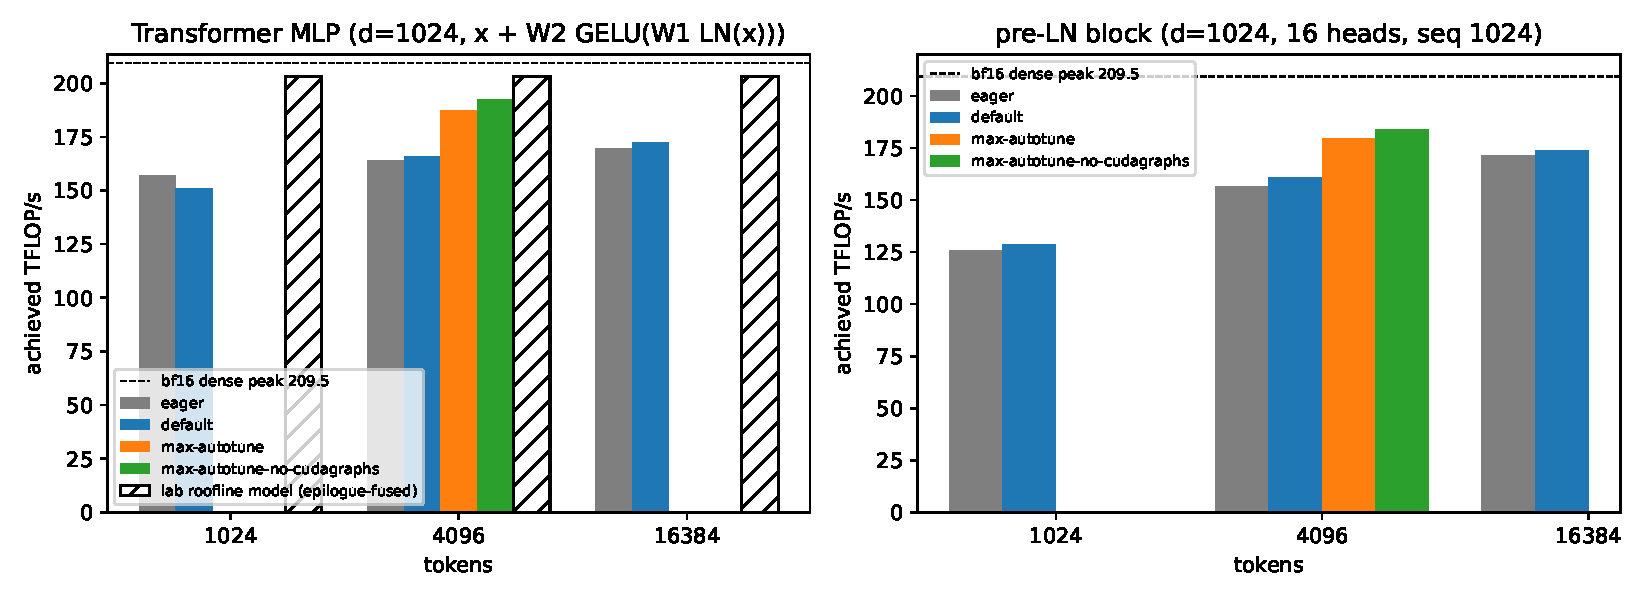
\includegraphics[width=\linewidth]{gpu_mlp_block.pdf}
\caption{MLP 与 block 的达到 TFLOP/s。MLP 图中的斜线柱是实验室 roofline 模型（epilogue 融合）预测的吞吐。GEMM 占主导时，所有版本都在 126--193 TFLOP/s（峰值的 60--92\%），留给融合的只有剩下的 10--15\%。最低的是 1024 token 的 block，因为 attention 和小 GEMM 的占比更大。}
\label{fig:mlp}
\end{figure}

\paragraph{手写 Triton vs Inductor。}既然 Inductor 在访存受限链上已经顶到带宽墙，手写 kernel 还有没有意义？\Cref{fig:triton} 给出了对比。
大尺寸（$16384\times4096$）上，手写 RMSNorm 用 162.3 µs，Inductor 175.0 µs，eager 1725.3 µs。bias+GELU 上手写和 Inductor 几乎一样（176.1 vs 175.6 µs），都在 1.52--1.53 TB/s。
所以对逐元素和行归约这类算子，Inductor 生成的 kernel 与手写 kernel 只差 0--7\%。手写的价值在于控制权，比如让整行驻留在寄存器里、绕开 Inductor 的 guard，而不在于更高的带宽上限。
小尺寸下比的是 launch 下限：手写 kernel 约 16--20 µs（主要是 Triton 的 Python launcher），Inductor 约 23--25 µs，eager 单个 kernel 约 11.8 µs。

\begin{figure}[H]
\centering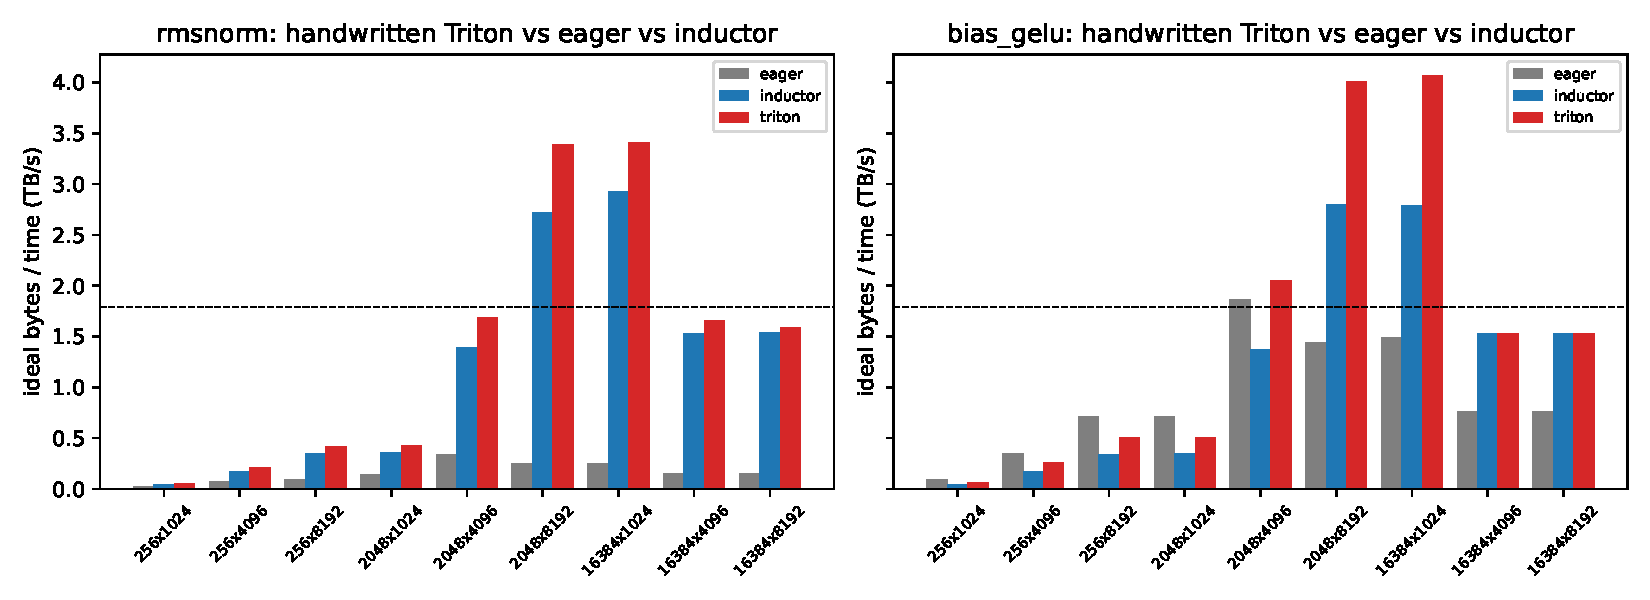
\includegraphics[width=\linewidth]{gpu_triton_fused.pdf}
\caption{手写 Triton 融合 kernel 与 eager、Inductor 的达到带宽（\texttt{fusion\_triton.jsonl}）。$16384\times1024$ 与 $2048\times8192$ 时数据只有 32 MB，落在 L2 里，手写 bias+GELU 达到 4.01--4.07 TB/s，这是 L2 带宽的量级。}
\label{fig:triton}
\end{figure}

\paragraph{编译成本与动态 shape。}上面的加速都是“编译好之后”的稳态。实际部署里，序列长度会变，每变一次都可能触发重编译。
为了看这笔账，我们对同一个 MLP 依次喂 10 个不同的序列长度（512, 768, 1024, 1536, 2048, 3072, 4096, 640, 1024, 2048），比较三种策略（\cref{fig:compile}）：

\begin{table}[H]
\centering\small
\begin{adjustbox}{max width=\linewidth}\begin{tabular}{lrrl}
\toprule
策略 & 编译出的图 & 首调用总耗时 & 说明 \\
\midrule
\texttt{dynamic=False} & 8 & 4.46 s & 每遇到新长度就重编译，直到 \texttt{cache\_size\_limit}=8 \\
默认（automatic dynamic） & 2 & 0.99 s & 第 1 次按静态编译，第 2 次发现长度变了，改编一个符号形状图 \\
\texttt{mark\_dynamic(x, 0)} & 1 & 0.54 s & 一开始就编符号形状图 \\
\bottomrule
\end{tabular}\end{adjustbox}
\caption{动态 shape 的重编译代价（\texttt{fusion\_dynamic.jsonl}）。}
\end{table}

三种策略的稳态时间是一样的：4096 token 时 static 419.8 µs，automatic 420.4 µs，mark\_dynamic 420.2 µs，eager 425.7 µs。
也就是说，对 GEMM 主导的模型，符号形状图没有可见的性能损失，而静态策略把 3.9 s 白白花在了 7 次重编译上。
工程上的做法因此很明确：serving 里会变化的长度维度应该 \texttt{mark\_dynamic}，或者把长度 pad 到少数几个 bucket。

\begin{figure}[H]
\centering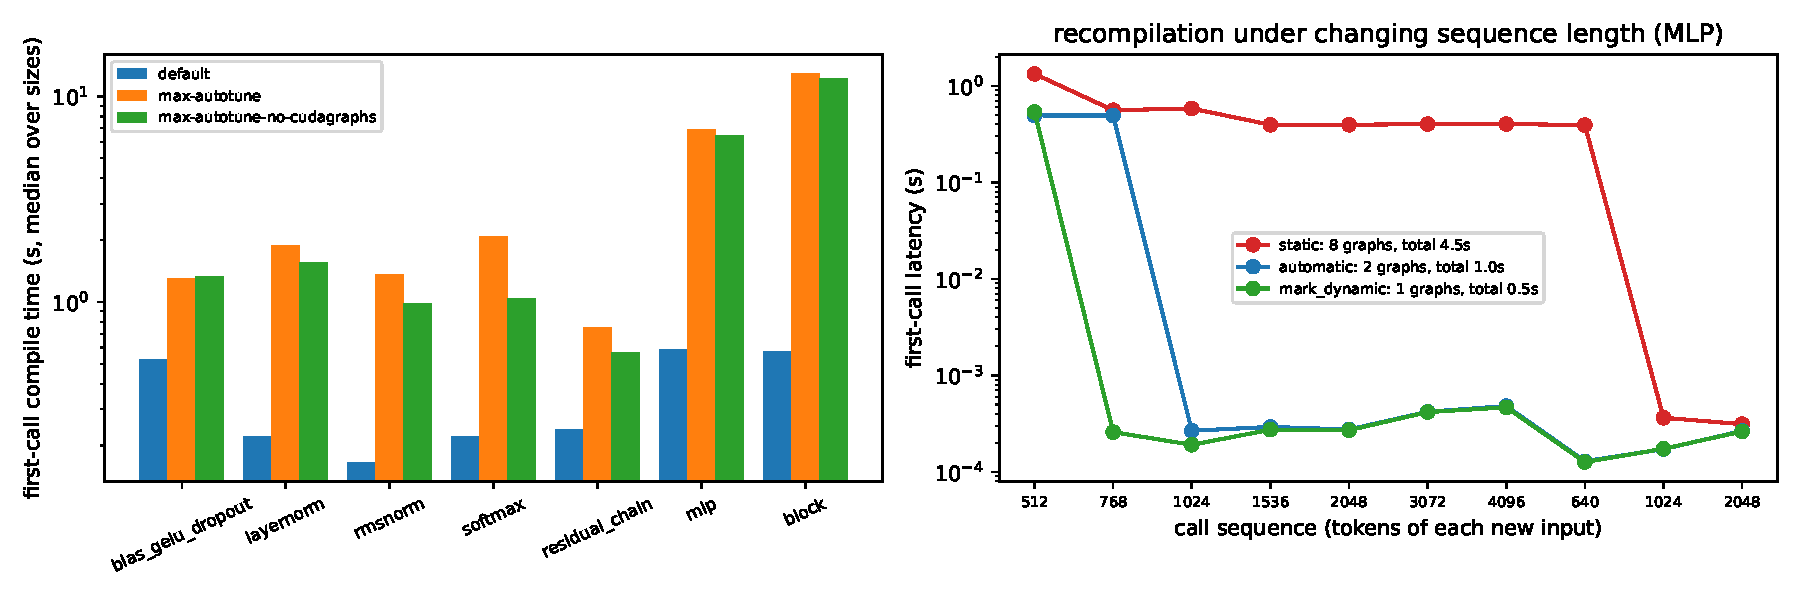
\includegraphics[width=\linewidth]{gpu_compile_dynamic.pdf}
\caption{左：各模式首次调用的编译时间（各尺寸取中位数，对数轴）。逐元素链 default 要 0.17--0.52 s，max-autotune 要 0.75--2.1 s；MLP/block 的 max-autotune 要 6.9/12.9 s，因为它要 benchmark 约 20 个 GEMM 模板，其中不少需要 128--144 KB 共享内存，在 sm\_120 的 99 KB 上直接失败。右：动态 shape 序列中每次首调用的延迟。}
\label{fig:compile}
\end{figure}

\subsection{Q2：调度/分块搜索——实测地形 vs 代价模型}

融合决定“哪些算子放进一个 kernel”，调度决定“这个 kernel 怎么切块、怎么排循环”。对 matmul 来说，后者几乎决定了一切。
TVM 和 Ansor 的做法是在很大的调度空间里搜索。这一节先看搜索本身的效率，再看真实 GPU 上的性能地形长什么样，最后问解析代价模型能不能代替实测。

\paragraph{CPU 模型。}实验室的 2048$^3$ 调度空间有 6 种循环序 $\times$ 8$^3$ 种 tile，共 3072 个调度。在单个 H100 SM 的代价模型下，只有 8 个落在最优的 5\% 以内。
\Cref{fig:cpu-sched} 比较了找到这样一个调度要评估多少次：按枚举顺序的 grid 要 434 次；random 中位 244 次（P90 为 649）；进化搜索中位 147.5 次（P90 为 496），比 random 快约 1.65$\times$。
最优调度是 ijk/256$\times$256$\times$64，5.99 ms，离 2.29 ms 的计算下限还很远。原因是 C 块的强度 $t_mt_n/(t_m+t_n)=128$ FLOP/B，低于这个模型的脊点 295。

\begin{figure}[H]
\centering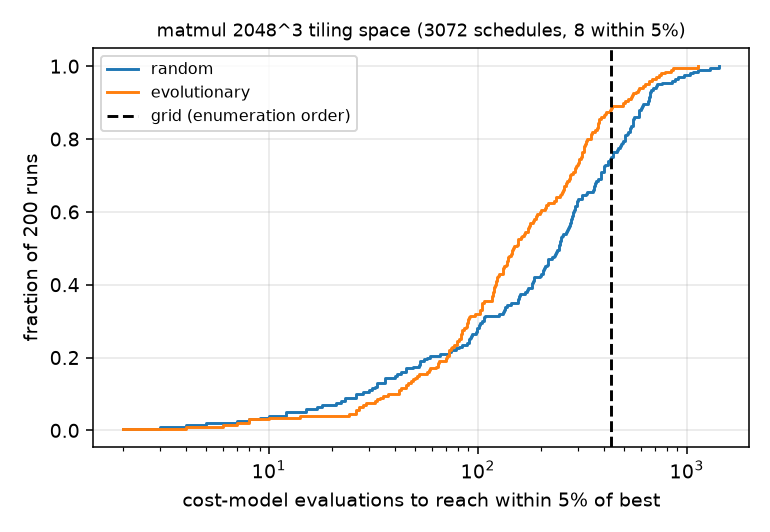
\includegraphics[width=0.62\linewidth]{schedule_search.png}
\caption{（CPU 模型）200 次重复中，达到最优 5\% 以内所需评估次数的 CDF（\texttt{schedule\_runs.csv}）。曲线越靠左，搜索越省。}
\label{fig:cpu-sched}
\end{figure}

\paragraph{GPU 实测地形。}换到真实 GPU，我们在三个形状上扫完整个 Triton 网格，结果见 \cref{tab:mm} 与 \cref{fig:mm-heat,fig:mm-land}。

\begin{table}[H]
\centering\small
\begin{adjustbox}{max width=\linewidth}\begin{tabular}{lrrrr}
\toprule
形状（fp16） & cuBLAS & 网格最优（配置） & autotune（选中配置） & 5\% 内配置数 / 可运行数 \\
\midrule
$4096^3$ & 209.6 & 211.8（64$\times$64$\times$64, w4, s3） & 206.7（64$\times$128$\times$32, w4, s4） & 29 / 176 \\
$8192^3$ & 214.3 & 221.5（128$\times$128$\times$32, w4, s3） & 214.7（128$\times$256$\times$64, w8, s3） & 17 / 96 \\
$256\times4096\times4096$ & 175.0 & 165.0（128$\times$64$\times$64, w8, s4） & 152.3（128$\times$64$\times$32, w4, s4） & 8 / 176 \\
\bottomrule
\end{tabular}\end{adjustbox}
\caption{Triton matmul 网格（TFLOP/s，\texttt{matmul\_search.jsonl}）。$8192^3$ 跳过了 $B_M$ 或 $B_N{=}32$ 的配置，它们不可能有竞争力，而且每个要跑数秒。$4096^3$ 上有 16 个 OOR 配置，全部是 $B_K{=}64$、stages 3--4 的大 tile，需要 110--196 KB 共享内存，超过了 99 KB。}
\label{tab:mm}
\end{table}

\begin{findingbox}[：一个 30 行的 Triton kernel 可以追平 cuBLAS，但最优 tile 随形状变化]
方阵上网格最优比 cuBLAS 快 1.0\%（$4096^3$）和 3.4\%（$8192^3$）；但三个形状的最优 tile 各不相同，只在 10 个候选里挑的 autotune 因此总是落后于网格最优。
\end{findingbox}

221.5 TFLOP/s 甚至高于规格表上的 209.5 TFLOP/s。这说明实卡运行在高于标称 boost 的频率上，“峰值”应该以实测为准。
最优 tile 的差别有清楚的解释。$4096^3$ 偏好 64$\times$64：这样有 $64\cdot64=4096$ 个 C 块，约 24.1 波，最后一波不满造成的浪费小。$8192^3$ 偏好 128$\times$128，瘦长的 $M{=}256$ 偏好 128$\times$64。
autotune 的 10 个教程候选覆盖不到这些变化，所以在方阵上落后网格最优 2.4--3.1\%，在瘦长形状上落后 7.7\%，比 cuBLAS 慢 13\%。

热力图把“为什么大 tile 不一定好”看得更清楚：

\begin{figure}[H]
\centering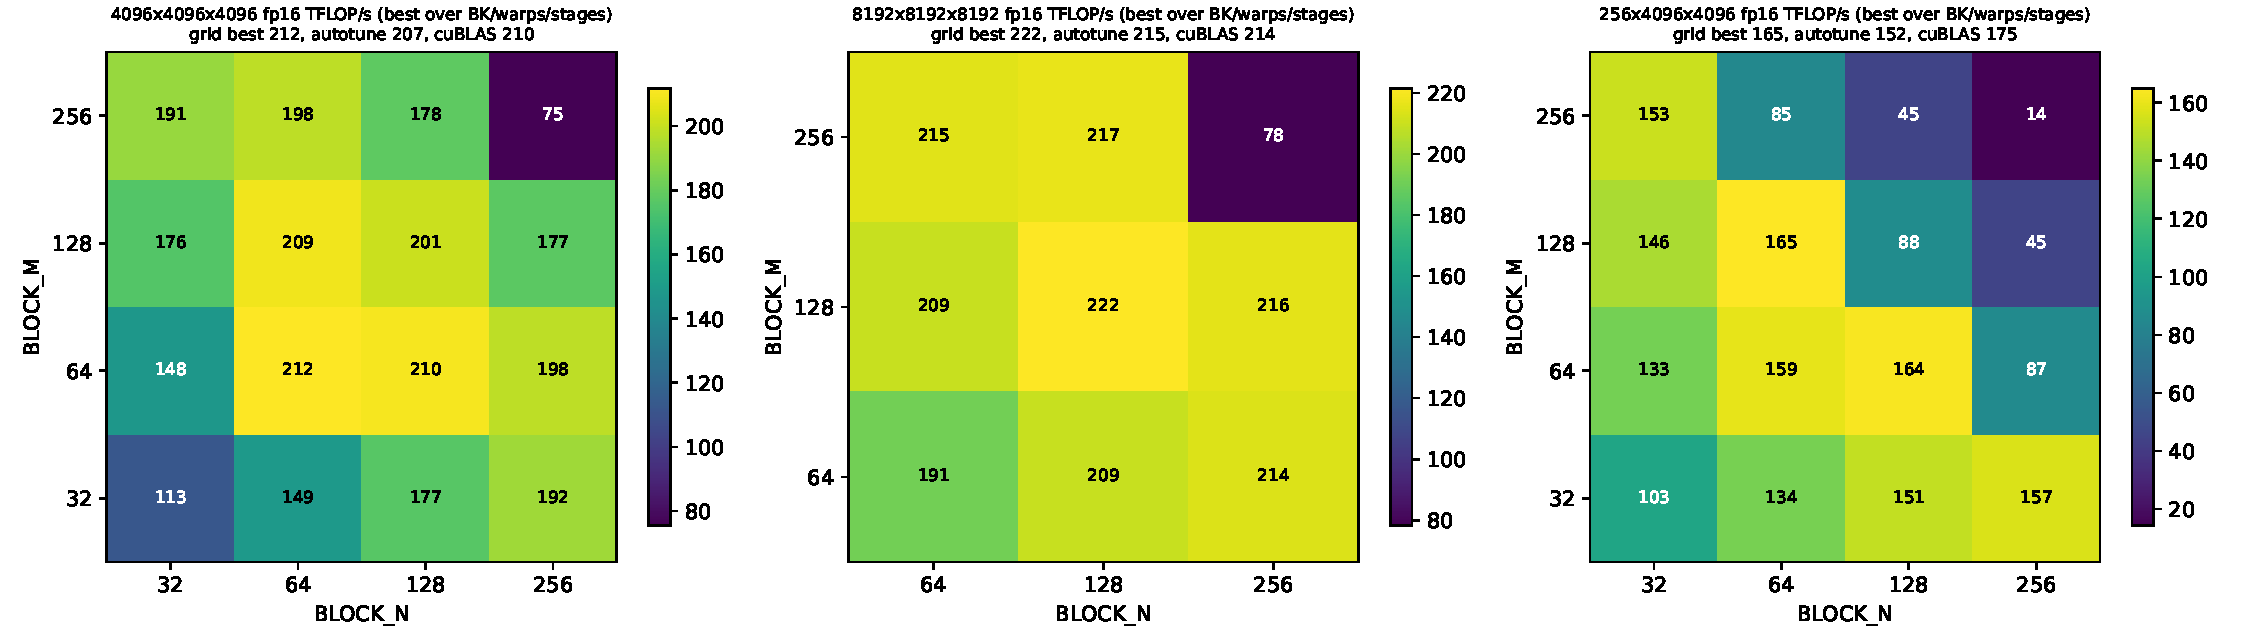
\includegraphics[width=\linewidth]{gpu_matmul_heatmap.pdf}
\caption{$B_M\times B_N$ 热力图（对 $B_K$/warps/stages 取最好值）。256$\times$256 一格在三个形状上都是最差（75/78/14 TFLOP/s），原因有两个：每个 program 的累加器是 $256\times256$ 的 fp32，需要 256 KB 寄存器，4--8 个 warp 装不下，发生寄存器溢出；而且只能切出 256 个（$4096^3$）甚至 16 个（$M{=}256$）C 块，170 个 SM 用不满。}
\label{fig:mm-heat}
\end{figure}

\begin{figure}[H]
\centering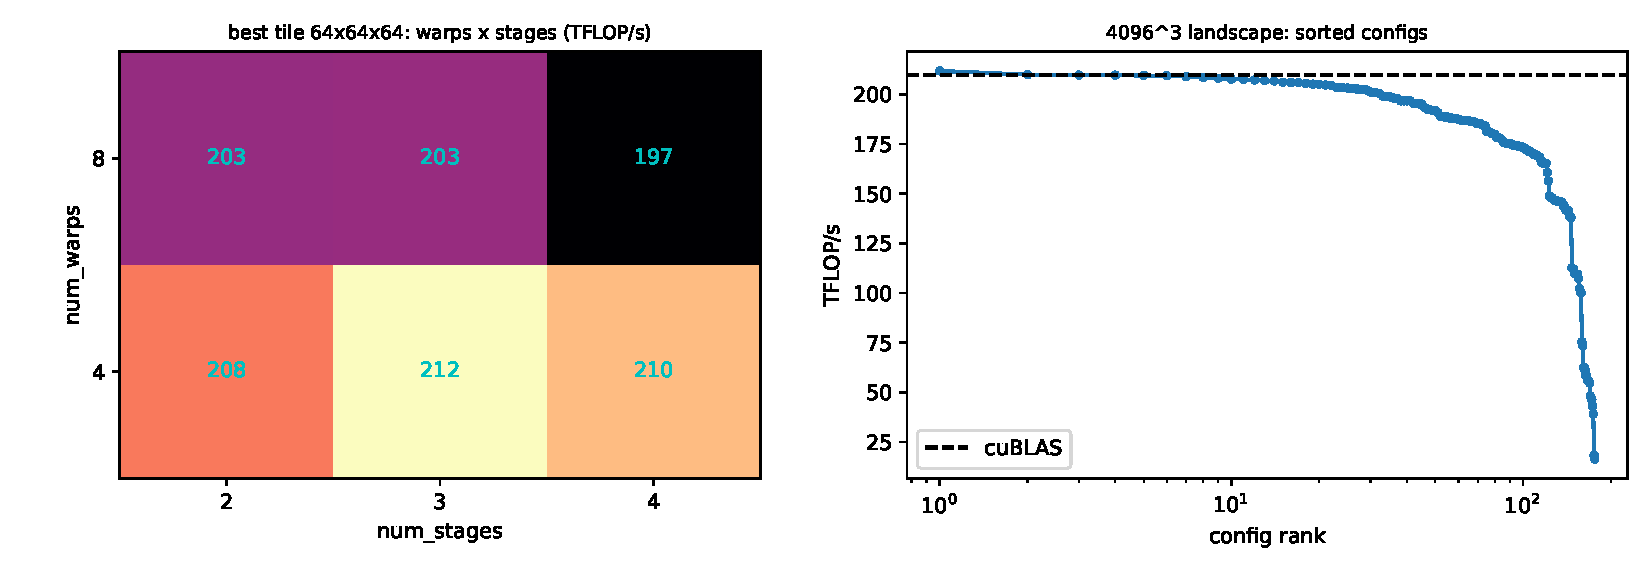
\includegraphics[width=\linewidth]{gpu_matmul_landscape.pdf}
\caption{左：在 $4096^3$ 的最优 tile（64$\times$64$\times$64）上，warps 与 stages 的影响。右：176 个可运行配置按吞吐排序，中位数 175.2 TFLOP/s，只有 29 个在最优的 5\% 以内。地形的顶部很窄，随手选一个配置大概率会掉下来。}
\label{fig:mm-land}
\end{figure}

\paragraph{代价模型能否排对？}实测地形这么陡，就引出一个实际问题：能不能用解析模型代替实测，先把好配置挑出来？\Cref{fig:costmodel} 与下表给出两个模型在 $(B_M,B_N,B_K)$ 三元组上的 Spearman 相关，以及各自选中的配置实际跑出多少。

\begin{table}[H]
\centering\small
\begin{tabular}{lrrrr}
\toprule
形状 & 实验室模型 $\rho$ & 实验室模型选中（实测） & 波次 roofline $\rho$ & 波次 roofline 选中（实测） \\
\midrule
$4096^3$ & 0.65 & 128$\times$256$\times$32（174.0） & 0.26 & 256$\times$256$\times$32（75.5） \\
$8192^3$ & 0.36 & 128$\times$256$\times$32（211.4） & 0.21 & 256$\times$256$\times$32（78.2） \\
$256\times4096^2$ & 0.10 & 128$\times$256$\times$32（44.1） & 0.72 & 64$\times$128$\times$32（151.7） \\
\bottomrule
\end{tabular}
\caption{两个解析代价模型的排序相关，以及它们选中配置的实测 TFLOP/s（\texttt{summary\_gpu.json}）。}
\end{table}

\begin{findingbox}[：每个解析模型只看见了一种效应]
实验室模型看见了数据复用，却看不见 SM 占用；波次 roofline 看见了 SM 占用，却看不见寄存器容量。所以解析模型适合剪掉明显不行的配置，最终排序还得靠实测或学习型模型。
\end{findingbox}

实验室模型只考虑数据复用和缓存容量。方阵上的主要矛盾恰好是“小 tile 复用低”，所以它在 $4096^3$ 上排得还行（$\rho=0.65$）。
但它对 $M{=}256$ 几乎没有信息（$\rho=0.10$），选中的 128$\times$256 只跑到 44.1 TFLOP/s：它不知道 $256\times4096$ 只能切出 2$\times$16 = 32 个 C 块，170 个 SM 只用上了 19\%。
波次 roofline 正好相反。它抓住了 SM 占用，在瘦长形状上 $\rho=0.72$；但它不建模寄存器，于是在方阵上选中了会寄存器溢出的 256$\times$256（75.5 TFLOP/s）。
两个模型都不理解 warps 和 stages（即流水线深度和寄存器分配），而实测最优 5\% 以内的候选恰恰在这两维上拉开差距。
这也解释了 Ansor/TVM 为什么用\emph{学习型}代价模型加真机测量：解析模型可以先去掉 OOR 和明显过小的 tile，但不适合做最后的排序。

\begin{figure}[H]
\centering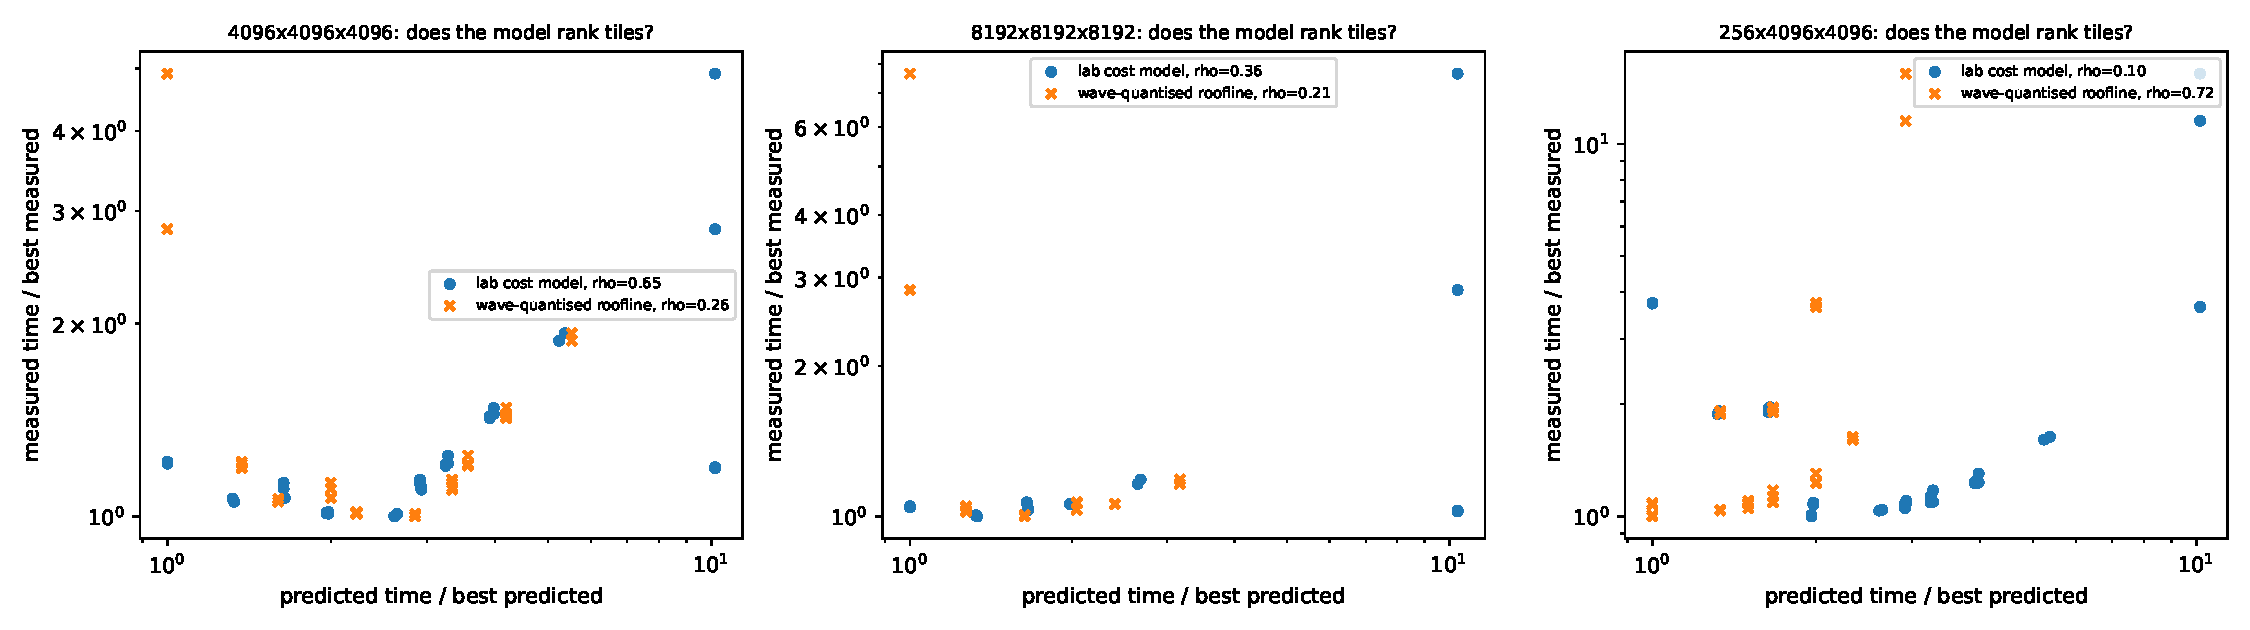
\includegraphics[width=\linewidth]{gpu_costmodel_rank.pdf}
\caption{预测时间（相对模型最优）对实测时间（相对实测最优），对数轴。理想的模型应该给出一条单调曲线，实际的点散得很开。右上角的离群点是实验室模型判为“工作集超出缓存”的 tile（预测慢 10$\times$），实测它们也确实是最差的一批，说明这个模型擅长排除坏配置。}
\label{fig:costmodel}
\end{figure}

\subsection{Q3：量化——精度与速度}

量化要同时回答两个问题：精度掉多少，速度快多少。这两个问题的答案往往来自不同的地方，精度取决于离群值和量化粒度，速度取决于读了多少字节、用了哪种 tensor core。
所以这一节先看精度，再分开看 GEMM 和 GEMV 的速度。

\paragraph{CPU 模型。}合成实验给出了两条预测，后面会在 GPT-2 上逐一检验。
\Cref{fig:cpu-quant} 在 1024 个通道中注入 8 个 50$\times$ 的离群通道，结果 per-tensor W8A8 的输出误差为 10.2\%，per-token 为 5.17\%，SmoothQuant $\alpha{=}0.5$ 为 1.99\%，LLM.int8 为 0.49\%。
另一组实验看 GPTQ：输入谱衰减为 1.0 时，GPTQ 的测试误差是 3.5\%（RTN 为 25.3\%）；输入各向同性时，GPTQ 反而更差（28.2\% vs 26.4\%）。
由此得到的预测是：(1) 离群值按\emph{通道}出现；(2) GPTQ 的收益取决于输入之间有没有相关性。

\begin{figure}[H]
\centering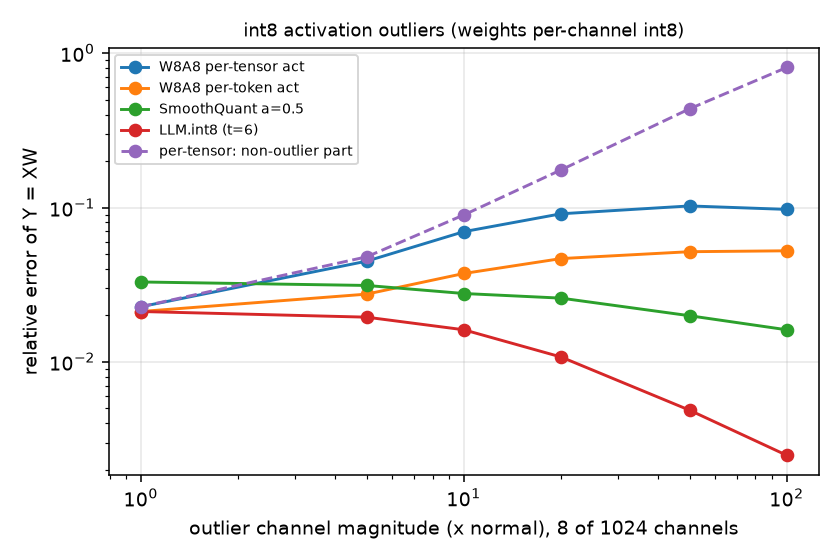
\includegraphics[width=0.8\linewidth]{quant_outliers.png}
\caption{（CPU 模型）激活离群倍数对各 W8A8 方案输出误差的影响（\texttt{quant\_outliers.csv}）。离群越强，per-tensor 越早失效。}
\label{fig:cpu-quant}
\end{figure}

\paragraph{GPU 实测：GPT-2 困惑度。}\Cref{tab:ppl} 是所有方法在两个 GPT-2 上的困惑度，\cref{fig:quant-ppl} 是同一组数据的图。表按位宽从高到低排，读的时候可以看每往下一档，哪些方法开始拉开差距。

\begin{table}[H]
\centering\small
\begin{adjustbox}{max width=\linewidth}\begin{tabular}{llrrrr}
\toprule
类别 & 方法 & 位宽 & GPT-2 124M & GPT-2 355M & 量化耗时（355M） \\
\midrule
基线 & fp16 & 16 & 29.96 & 21.72 & -- \\
\midrule
\multirow{2}{*}{int8 RTN} & per-tensor & 8 & 34.33 & 23.40 & 即时 \\
 & per-channel & 8 & 29.98 & 21.72 & 即时 \\
\midrule
\multirow{4}{*}{int4} & RTN per-channel & 4 & 38.40 & 25.54 & 即时 \\
 & GPTQ per-channel & 4 & 32.59 & 23.19 & 36.5 s \\
 & RTN g128 & 4 & 33.27 & 23.04 & 即时 \\
 & AWQ 式 g128 & 4 & 32.36 & 23.00 & 23.4 s \\
 & GPTQ g128 & 4 & \textbf{31.20} & \textbf{22.53} & 36.6 s \\
\midrule
\multirow{3}{*}{int3 g128} & RTN & 3 & 65.92 & 32.45 & 即时 \\
 & AWQ 式 & 3 & 53.35 & 29.43 & 23.4 s \\
 & GPTQ & 3 & \textbf{37.24} & \textbf{25.50} & 36.5 s \\
\midrule
\multirow{7}{*}{W8A8（模拟）} & 激活 per-tensor & 8 & 49.94 & 23.97 & -- \\
 & 激活 per-token & 8 & 30.18 & 21.79 & -- \\
 & SmoothQuant $\alpha{=}0.5$ + per-tensor & 8 & 407.25 & 26.53 & 1.1 s \\
 & SmoothQuant $\alpha{=}0.8$ + per-tensor & 8 & 30.49 & 21.97 & 1.1 s \\
 & SmoothQuant $\alpha{=}0.5$ + per-token & 8 & 30.15 & 21.91 & 1.1 s \\
 & SmoothQuant $\alpha{=}0.8$ + per-token & 8 & 30.16 & 21.77 & 1.1 s \\
 & LLM.int8（阈值 6） & 8 & \textbf{30.06} & \textbf{21.77} & -- \\
\bottomrule
\end{tabular}\end{adjustbox}
\caption{wikitext-2 test 困惑度（286,720 个评估 token，\texttt{quant\_ppl\_gpt2*.jsonl}）。量化范围是所有 block 内的线性层；嵌入与 lm\_head 保持 fp16。}
\label{tab:ppl}
\end{table}

\begin{findingbox}[：位宽越低，“用数据”的方法越值钱]
int8 per-channel 的朴素取整（RTN）已经无损；越往低位走，用校准数据的 GPTQ 领先越多，到 int3 时它把 124M 的困惑度从 65.92 拉回 37.24。
\end{findingbox}

逐档来看。int8 per-channel 几乎没有损失（29.98 vs 29.96；21.72 vs 21.72），per-tensor 则损失 4.4/1.7 ppl，这和 CPU 实验里“重尾权重让 per-tensor 失效”一致。
到 int4 g128，RTN 损失 3.3/1.3 ppl，GPTQ 把损失压到 1.24/0.81。到 int3，AWQ 式缩放只能到 53.35，远不如 GPTQ 的 37.24。
有一个对比特别能说明误差补偿的作用：GPTQ per-channel（32.59）比 RTN g128（33.27）还好，也就是说，补偿误差抵得上多用 16 倍的 scale。
另外，模型越大越耐量化：355M 在 int3 GPTQ 下只损失 3.8 ppl，124M 损失 7.3 ppl。

W8A8 那几行里有一个异常值：SmoothQuant $\alpha{=}0.5$ 加 per-tensor 激活，124M 的困惑度是 407.25。

\begin{findingbox}[：SmoothQuant 的迁移强度 $\alpha$ 是模型相关的超参数]
同样是 per-tensor 激活，$\alpha{=}0.5$ 让 GPT-2 124M 崩到 407.25，比完全不平滑的 49.94 还差 8$\times$；换成 $\alpha{=}0.8$ 就降到 30.49，只损失 0.53。
\end{findingbox}

355M 上是同样的趋势：$\alpha{=}0.5$ 比不平滑更差（26.53 vs 23.97），$\alpha{=}0.8$ 恢复到 21.97。
原因藏在公式 $s_j=\max|X_j|^\alpha/\max|W_j|^{1-\alpha}$ 里。$\alpha$ 较小时，$s_j$ 对 $\max|W_j|$ 更敏感：如果某个输入通道的权重列很大、校准时的激活却很小，就会得到 $s_j\ll1$，
测试时这个通道的 $x_j/s_j$ 被放大，反而成了新的 per-tensor 离群值。SmoothQuant 原文对不同模型使用 0.5--0.85 的 $\alpha$，和这里的观察一致。
另外两点也值得记住。只要激活改成 per-token 量化，W8A8 的损失就降到 0.2/0.07 ppl。LLM.int8 最接近 fp16（30.06/21.77），代价是每层平均有 3.3/4.1 列、最多 50/60 列要走 fp16，计算变得不规则。

\begin{figure}[H]
\centering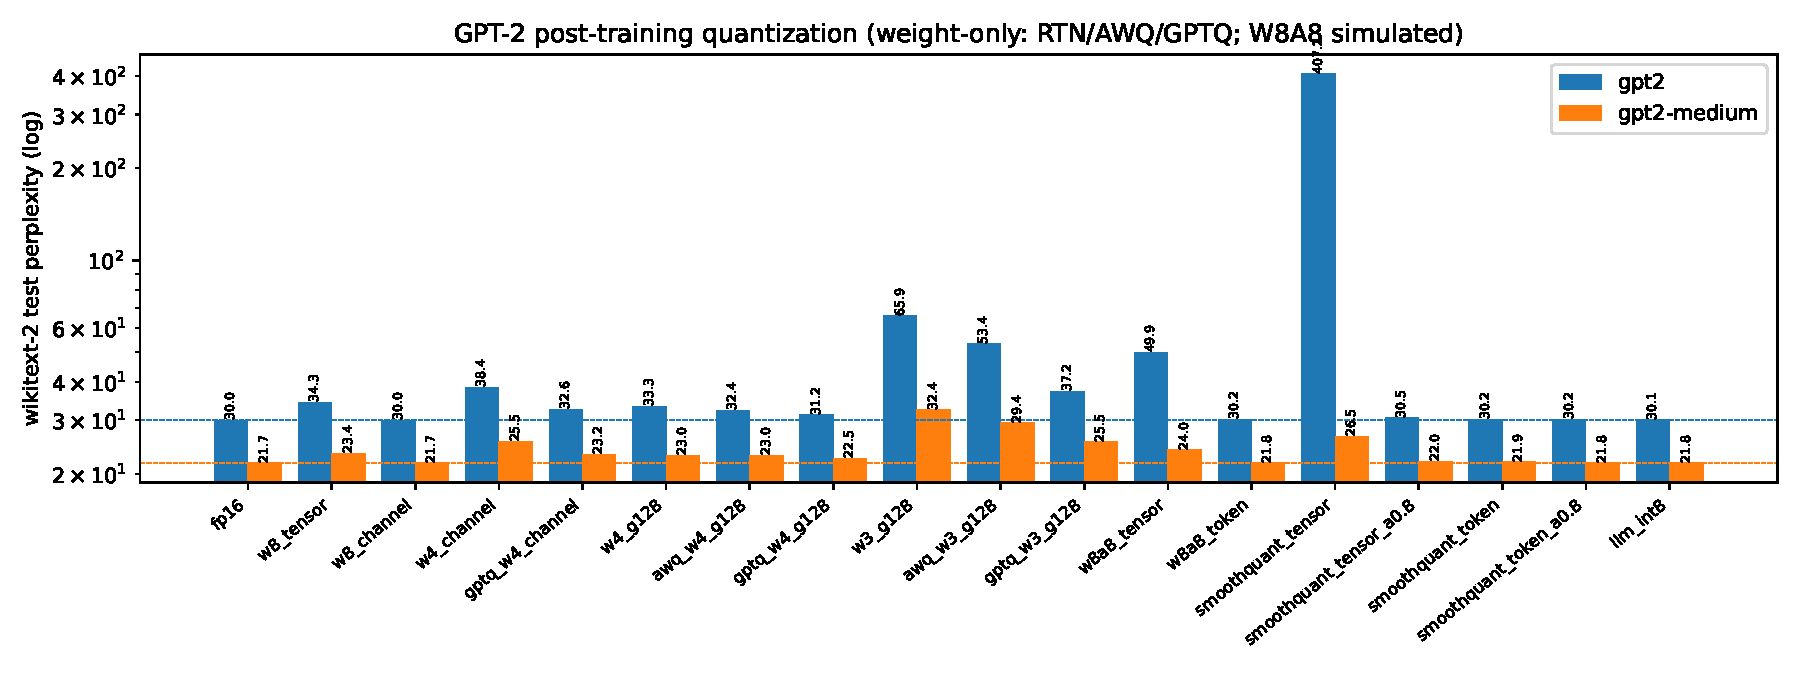
\includegraphics[width=\linewidth]{gpu_quant_ppl.pdf}
\caption{各量化方法的困惑度（对数轴，虚线为 fp16）。离虚线越远，损失越大；int3 RTN 与 $\alpha{=}0.5$ 的 per-tensor SmoothQuant 是两个最明显的失败。}
\label{fig:quant-ppl}
\end{figure}

\paragraph{激活离群统计。}前面的解释都假设 GPT-2 里有按通道出现的激活离群值。这里直接去数：在 16 个校准窗口上，统计每个线性层输入的逐通道 $\max|x|$（\cref{fig:outliers}）。
GPT-2 124M 最大的离群出现在第 2 个 block 的 \texttt{mlp.c\_proj} 输入（GELU 之后），为 62.8，而该层通道 $\max|x|$ 的中位数只有 1.60，相差 39$\times$。
355M 的最大离群在第 3 个 block 的 \texttt{mlp.c\_proj}，76.2 对中位数 1.78。
\texttt{c\_fc} 的输入（LN 之后）在多个 block 中都是同一个通道 138 最大（124M 第 2 block 为 19.9，第 5 block 为 11.2）。这对应文献中 GPT-2 残差流里那个固定的离群维度，经 LN 权重放大后的样子。
超过阈值 6 的通道平均每层 4.0 个（124M）和 5.9 个（355M），集中在靠后 block 的 \texttt{mlp.c\_proj}（355M 第 21--23 block 每层 65--68 个）。
这验证了 CPU 实验的前提：离群按通道出现，数量少（$<$2\%），幅度大。
不过，和 OPT-6.7B 之后出现的“系统性 $>$20$\times$ 离群”相比，GPT-2 的离群还算温和，所以朴素的 W8A8 per-token 已经接近无损；离群真正致命的是 per-tensor 激活量化。

\begin{figure}[H]
\centering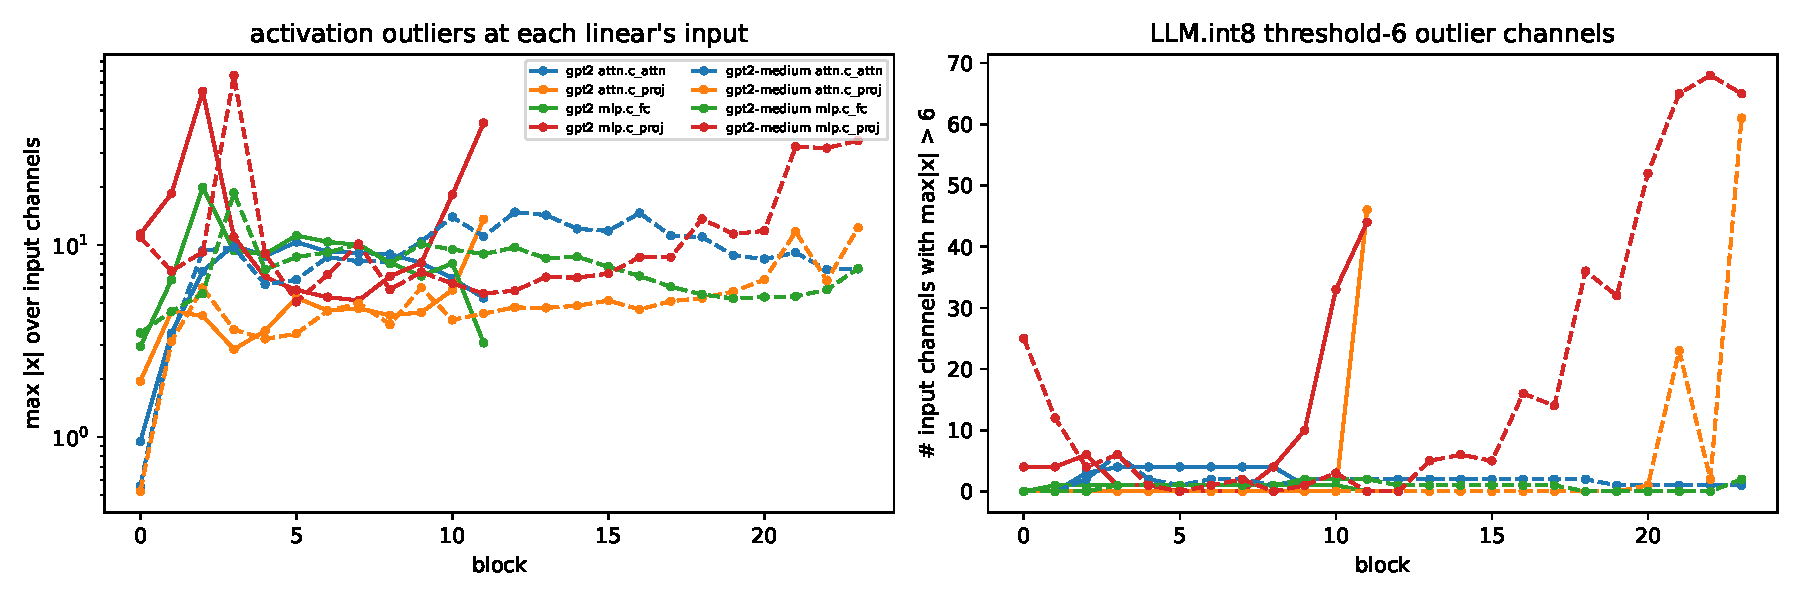
\includegraphics[width=\linewidth]{gpu_act_outliers.pdf}
\caption{左：每层输入的最大绝对激活（对数轴）；右：$\max|x|>6$ 的输入通道数，也就是 LLM.int8 会放到 fp16 的列数。实线为 124M，虚线为 355M。}
\label{fig:outliers}
\end{figure}

\paragraph{低精度 GEMM 吞吐。}精度之后看速度，先看大矩阵乘（\cref{fig:lowprec}，\texttt{quant\_speed.jsonl}）。
正确性先确认过：int8 结果与 fp64 参考逐元素完全相等（\texttt{exact=true}）；FP8 e4m3 相对 fp32 参考的误差为 $1.66\times10^{-3}$。

\begin{table}[H]
\centering\small
\begin{tabular}{lrrrrrr}
\toprule
$[M\times4096]\times[4096\times16384]$ & bf16 TFLOP/s & int8 TOP/s & fp8 TFLOP/s & int8/bf16 & fp8/bf16 \\
\midrule
$M{=}32$（decode 式） & 47.7 & 271.9 & 221.1 & 5.70$\times$ & 4.64$\times$ \\
$M{=}128$ & 88.7 & 584.9 & 341.6 & 6.59$\times$ & 3.85$\times$ \\
$M{=}1024$ & 177.4 & 599.9 & 383.0 & 3.38$\times$ & 2.16$\times$ \\
$M{=}8192$（prefill 式） & 226.9 & 679.4 & 456.2 & 2.99$\times$ & 2.01$\times$ \\
\bottomrule
\end{tabular}
\caption{低精度 GEMM 吞吐（N=16384, K=4096）。}
\end{table}

\begin{findingbox}[：在 GeForce Blackwell 上 int8 是 bf16 的 3 倍，不是 2 倍]
大 $M$ 时 int8、FP8、bf16 的吞吐之比约为 3:2:1（679.4 TOP/s、456.2 TFLOP/s、226.9 TFLOP/s），因为这张 GeForce 卡的 bf16 在 fp32 累加时只有半速。
\end{findingbox}

按规格，bf16 在 fp32 累加下是 209.5 TFLOP/s；int8（int32 累加）是满速，规格 838 TOP/s，实测达到 81\%；FP8 经 \texttt{\_scaled\_mm} 也用 fp32 累加，规格 419 TFLOP/s。
数据中心卡（H100）上则不同，FP8 与 int8 都是 bf16 的 2$\times$。所以“int8 比 bf16 快多少”这个问题，答案取决于具体的卡。
小 $M$ 时比例更大（$M{=}32$ 时 int8 是 bf16 的 5.7$\times$），但原因不一样。bf16 的 cuBLAS 在 $M{=}32$ 选了一个低效的 kernel（47.7 TFLOP/s，90.0 µs），
而读 128 MB 权重在 1.79 TB/s 下的下限就有 75 µs，可见 bf16 在 decode 形状上本来就接近带宽墙。int8 只读一半字节（67 MB），实测 15.8 µs，其中部分命中了 L2。
因此 W8A8 在 decode 上的收益主要来自\emph{少读字节}，在 prefill 上来自\emph{更高的 tensor core 峰值}。

\begin{figure}[H]
\centering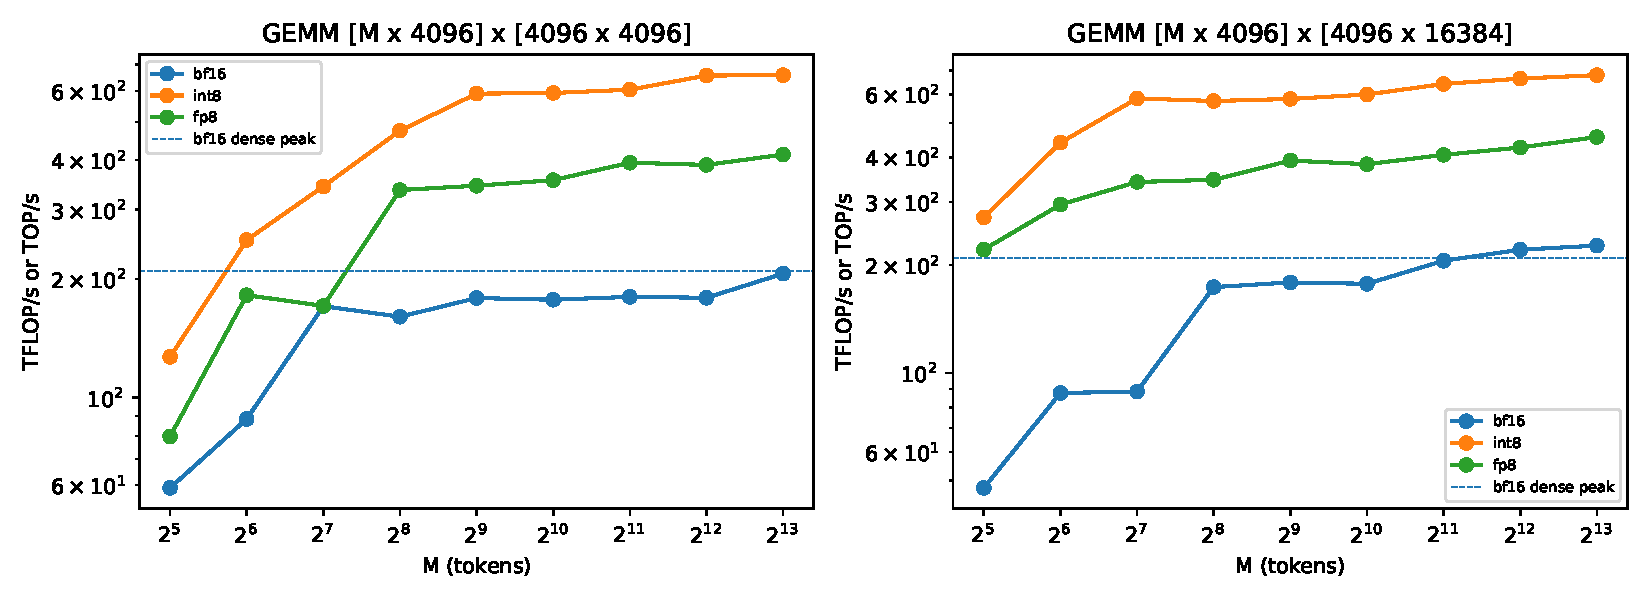
\includegraphics[width=\linewidth]{gpu_lowprec_gemm.pdf}
\caption{bf16 / int8 / FP8 GEMM 吞吐随 $M$ 的变化（log-log）。$N{=}K{=}4096$ 时 bf16 权重只有 32 MB，完全在 L2 里，所以小 $M$ 下的数字比“冷权重”乐观。}
\label{fig:lowprec}
\end{figure}

\paragraph{batch-1 weight-only：带宽说了算。}decode 时 batch 往往是 1，矩阵乘退化成矩阵乘向量（GEMV），每个权重只用一次，时间几乎全花在读权重上。
这种场景下 weight-only 量化的收益应该等于字节的缩减比例。\Cref{fig:gemv} 与下表检验这一点，数字以 cold 模式（轮换副本，工作集 $>$ 384 MB）为准：

\begin{table}[H]
\centering\small
\begin{adjustbox}{max width=\linewidth}\begin{tabular}{lrrrrr}
\toprule
权重 $N\times K$ & bf16 cuBLAS µs & W8A16 µs（加速） & W4A16 µs（加速） & 先反量化再 matmul µs & bf16 TB/s \\
\midrule
$4096\times4096$ & 25.5 & 16.6（1.54$\times$） & 17.3（1.47$\times$） & 267.2 & 1.31 \\
$11008\times4096$ & 57.3 & 28.6（2.00$\times$） & 21.3（2.69$\times$） & 1096.8 & 1.57 \\
$16384\times8192$ & 163.0 & 82.5（1.98$\times$） & 62.2（2.62$\times$） & 3688.2 & 1.65 \\
$32768\times8192$ & 319.5 & 178.9（1.79$\times$） & 142.0（2.25$\times$） & 7454.3 & 1.68 \\
\bottomrule
\end{tabular}\end{adjustbox}
\caption{batch 1 GEMV（cold），\texttt{quant\_speed.jsonl}。W8/W4 与各自反量化参考的相对误差为 $2.1\times10^{-4}$。}
\end{table}

\begin{findingbox}[：W8 接近 2$\times$、W4 只到 2.3--2.7$\times$，“先反量化”比融合 W4 kernel 慢 15--59$\times$]
W8A16 读一半字节，就快了接近 2$\times$；W4A16 离理论上限还差一截。而反量化如果不融合进 kernel，weight-only 量化不但不快，反而更慢。
\end{findingbox}

bf16 GEMV 在大矩阵上达到 1.65--1.68 TB/s，是规格峰值的 92--94\%，已经完全受带宽限制。W8A16 读一半字节，加速 1.79--2.00$\times$，接近理论的 2$\times$。
W4A16 的理论上限是 3.76$\times$（\cref{eq:w4bound}），我们的 Triton kernel 只做到 2.25--2.69$\times$，有效带宽 0.98--1.11 TB/s。
瓶颈已经从 DRAM 转到了解包（移位、掩码、int$\to$fp 转换）和 x 的跨步读取上。Marlin 等生产级 W4 kernel 在 dequant 指令排布上下了很多工夫，原因就在这里。
另一个极端是“先在 PyTorch 里把权重反量化成 fp16，再调 cuBLAS”：它比直接用 bf16 算还慢 10--23$\times$，因为要启动多个 kernel、产生 fp32 中间张量，反量化本身还要写出一整份 fp16 权重。
换句话说，weight-only 量化只有\emph{融合进 GEMV/GEMM kernel} 时才有速度收益。小矩阵（4096$^2$）是例外，三种方法都被 15--25 µs 的 launch 下限压平了。

\begin{figure}[H]
\centering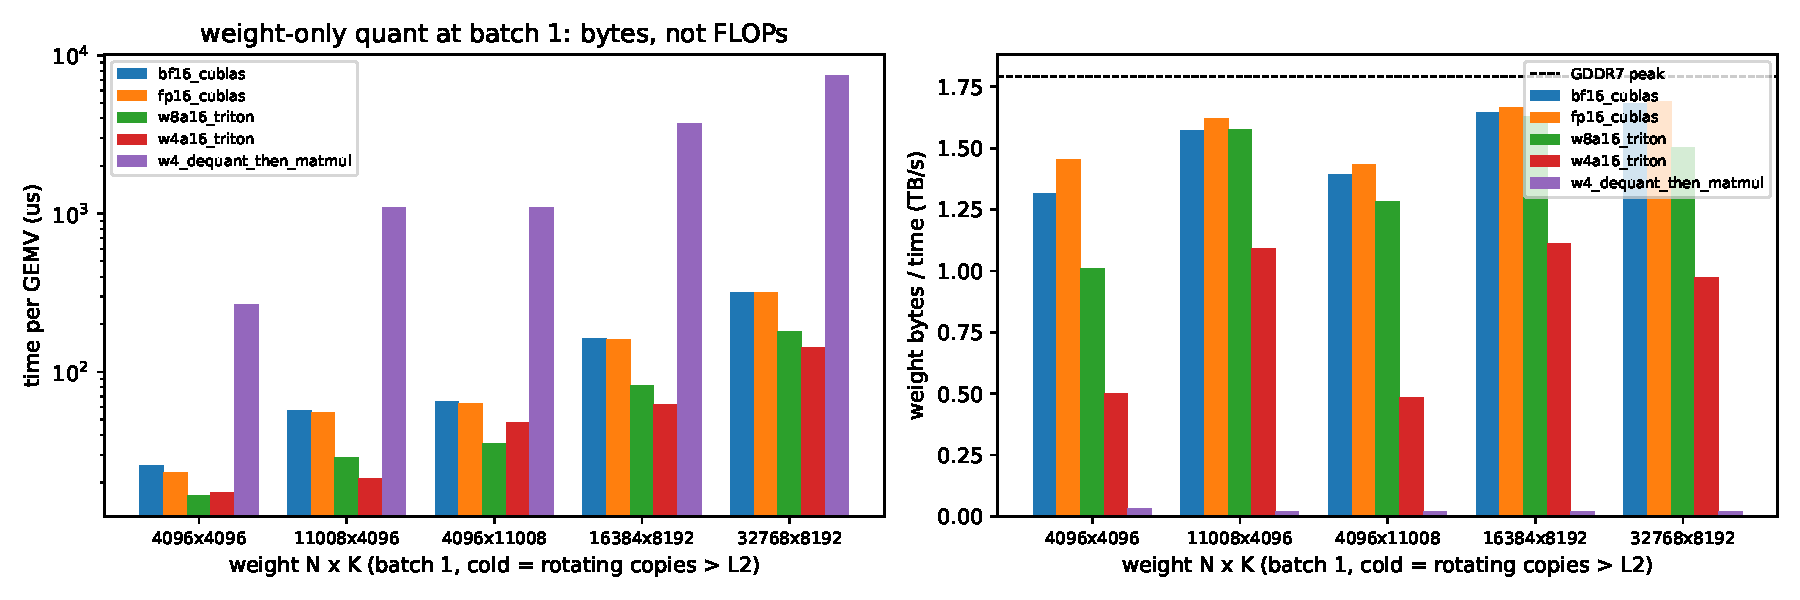
\includegraphics[width=\linewidth]{gpu_weight_only_gemv.pdf}
\caption{batch-1 GEMV 的时间（左，对数）与有效带宽（右，权重字节 / 时间），cold 模式。bf16 贴着带宽墙，W8 的时间随字节减半，W4 被解包开销拖住。}
\label{fig:gemv}
\end{figure}

\subsection{Q4：剪枝——精度与稀疏 kernel 速度}

剪枝面临和量化类似的两个问题，但难度更大：剪掉的权重不但会影响精度，而且只有当 GPU 真的能跳过这些零时，才会换来速度。

\paragraph{CPU 模型。}\Cref{fig:cpu-prune} 给出了合成实验的基线。在 1024$^2$ 的重尾矩阵上，非结构化 50\% 剪枝的输出误差为 20.4\%，2:4 为 29.0\%，4:8 为 25.1\%：结构约束越紧，误差越大。
小 MLP 上，幅值剪枝 90\% 且不微调时，准确率掉到 36.6\%；微调 3 轮回到 63.6\%（稠密为 66.2\%）。

\begin{figure}[H]
\centering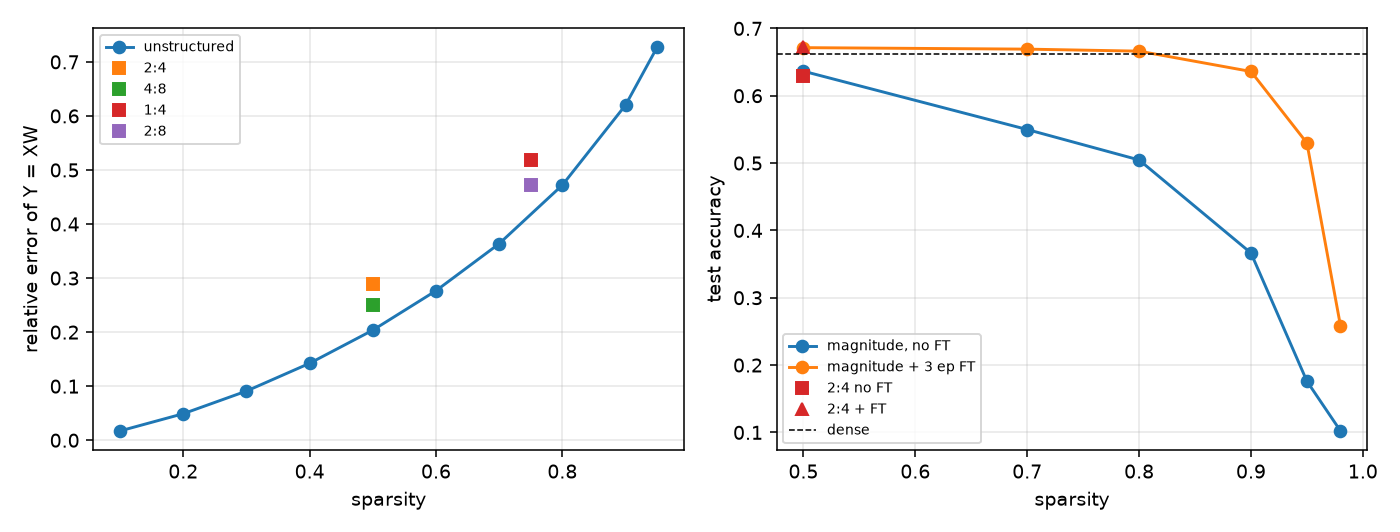
\includegraphics[width=0.85\linewidth]{pruning.png}
\caption{（CPU）左：剪枝方式对输出误差的影响；右：小 MLP 的稀疏度—准确率曲线，分含与不含微调两种（\texttt{pruning\_matrix.csv}、\texttt{pruning\_mlp.csv}）。}
\label{fig:cpu-prune}
\end{figure}

\paragraph{GPU 实测。}到 GPT-2 上，我们先看精度（\cref{tab:prune}），再看稀疏 kernel 的速度；两者的图都在 \cref{fig:prune}。

\begin{table}[H]
\centering\small
\begin{tabular}{lrr}
\toprule
方法（GPT-2 124M，一次性，无微调） & 稀疏度 & wikitext-2 ppl \\
\midrule
稠密 & 0 & 29.96 \\
幅值 30\% & 0.30 & 42.46 \\
幅值 50\% & 0.50 & 538.35 \\
幅值 70\% & 0.70 & 5698.52 \\
幅值 2:4 & 0.50 & 735.95 \\
幅值 4:8 & 0.50 & 346.51 \\
Wanda 50\%（按行） & 0.50 & \textbf{47.21} \\
Wanda 2:4 & 0.50 & \textbf{116.38} \\
\bottomrule
\end{tabular}
\caption{一次性剪枝的困惑度（\texttt{prune\_ppl\_gpt2.jsonl}）。Wanda 的分数 $|W_{ij}|\cdot\|X_j\|_2$ 来自 64 个校准窗口。}
\label{tab:prune}
\end{table}

\begin{findingbox}[：同样 50\%，“看激活”比“看权重”好 11 倍]
同样剪掉 50\%，幅值剪枝把困惑度从 29.96 推到 538.35，Wanda 只到 47.21，因为一个小权重乘上一个大激活并不小。
\end{findingbox}

2:4 时也是一样，幅值 735.95 对 Wanda 116.38。背后的原因和 \cref{fig:outliers} 相同：少数输入通道的激活比其他通道大几十倍，只看 $|W|$ 会把这些通道上的“小”权重剪掉。
N:M 约束越紧，精度越差（4:8 的 346.51 好于 2:4 的 735.95），方向与 CPU 实验的 25.1\% vs 29.0\% 一致。
即使是 Wanda 2:4，困惑度也涨了 3.9$\times$。GPT-2 这样的小模型冗余不多，生产中用 2:4 需要配合再训练（NVIDIA 的 ASP 流程）。

精度之外，剩下的问题是：剪出来的稀疏矩阵，GPU 算得快吗？

\begin{table}[H]
\centering\small
\begin{tabular}{lrrrr}
\toprule
$W$ 形状（fp16） & $M$ & 稠密 µs & 2:4 cuSPARSELt µs & 加速 \\
\midrule
$4096\times4096$ & 32 & 13.4 & 445.0 & 0.03$\times$ \\
$4096\times4096$ & 2048 & 346.8 & 456.9 & 0.76$\times$ \\
$4096\times4096$ & 8192 & 1244.8 & 806.6 & 1.54$\times$ \\
$16384\times4096$ & 2048 & 1246.4 & 801.2 & 1.56$\times$ \\
$16384\times4096$ & 8192 & 4936.4 & 3152.5 & 1.57$\times$ \\
$4096\times16384$ & 8192 & 4947.6 & 3128.2 & 1.58$\times$ \\
\bottomrule
\end{tabular}
\caption{2:4 半结构化稀疏 GEMM（\texttt{prune\_speed.jsonl}）。与稠密结果的相对误差 $\le 3.6\times10^{-4}$。CUTLASS 后端在 sm\_120 上报错 \emph{“Supported only on GPUs with compute capability 8.x”}，只有 cuSPARSELt 可用。}
\end{table}

\begin{findingbox}[：2:4 在大 GEMM 上兑现 1.54--1.58$\times$，小 $M$ 被约 445 µs 的固定开销吞掉]
2:4 稀疏只有在大 GEMM 上才变快，而且达不到理论的 2$\times$；在 decode 这类小 $M$ 场景下完全不能用。
\end{findingbox}

大形状上，cuSPARSELt 达到 340.8--351.5 有效 TFLOP/s（按稠密 FLOPs 计），即 1.54--1.58$\times$。没到 2$\times$ 的原因是元数据读取和压缩格式本身的额外开销。
但它每次调用有约 445 µs 的下限，而 $M{=}32$ 时稠密 GEMM 只要 13.4 µs，所以 $M\le2048$ 时 2:4 反而更慢。
非结构化的 CSR（cuSPARSE）更糟。在 $4096^2$、$M{=}512$ 上，50\% 稀疏时慢 18.5$\times$（1815.1 vs 98.1 µs），要到 99\% 稀疏才快 2.18$\times$；batch 1 时，任何稀疏度都不比稠密快（0.28--0.91$\times$）。
这就是 Deep Compression 时代“剪枝省存储”和今天 GPU 上“剪枝省时间”之间的鸿沟：要省时间，需要硬件认识的稀疏结构（2:4），还需要足够大的问题规模。

\begin{figure}[H]
\centering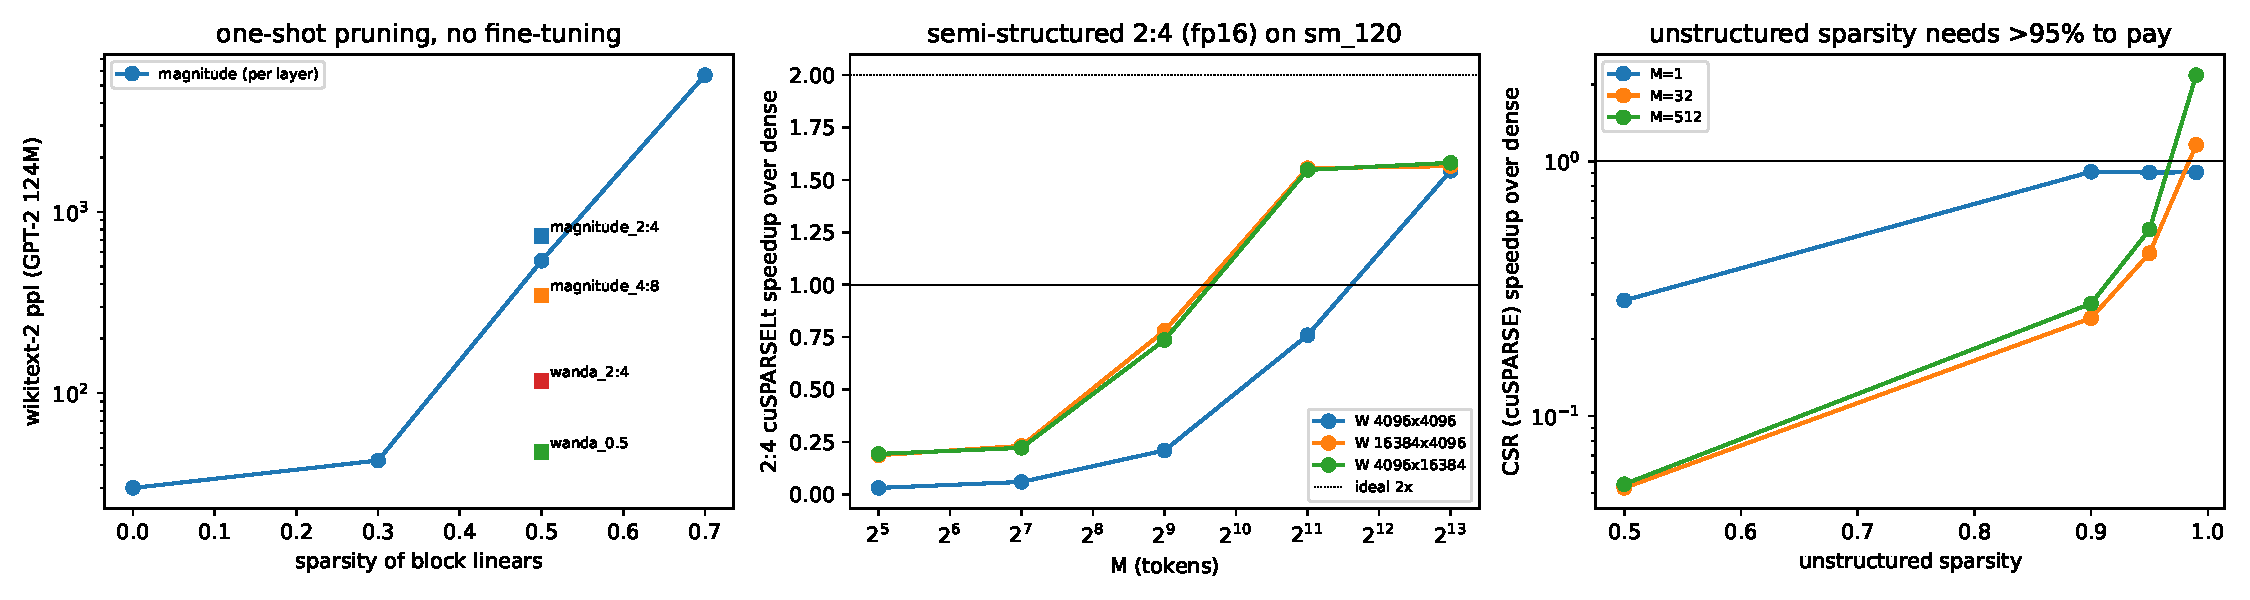
\includegraphics[width=\linewidth]{gpu_pruning.pdf}
\caption{左：GPT-2 一次性剪枝的困惑度（对数）；中：2:4 cuSPARSELt 相对稠密 cuBLAS 的加速随 $M$ 的变化，越过 1 的位置就是它开始划算的规模；右：CSR 相对稠密的加速随稀疏度的变化（$4096^2$）。}
\label{fig:prune}
\end{figure}

\subsection{Q5：LoRA 与 QLoRA-like 微调}

LoRA 常被概括为“只训练 1\% 的参数”。这一节要弄清楚的是：可训参数少了这么多，显存和时间到底省在哪里，又有哪些部分一点也省不掉。

\paragraph{CPU 模型。}先在单层上确认 LoRA 的数学。设 $d{=}256$，真实的 $\Delta W$ 秩为 8。$r{=}4$ 时拟合误差 0.434，接近 Eckart--Young 下界 0.424（秩为 $r$ 的最优近似误差）；$r{=}8$ 时误差降到 0.044。
可训参数是 4096，而全量是 65,536（6.25\%）。LoRA 初始化时输出与基座的最大差为 0，合并后最大差为 $3.3\times10^{-15}$（\texttt{lora\_fit.csv}、\texttt{lora\_params.csv}）。

\paragraph{GPU 实测（GPT-2 medium，wikitext-2，150 步，batch $8\times512$）。}下表汇总了各配置的成本与效果，曲线见 \cref{fig:lora-curves,fig:lora-cost}，原始数据在 \texttt{lora\_ft.jsonl}。

\begin{table}[H]
\centering\small
\begin{adjustbox}{max width=\linewidth}\begin{tabular}{lrrrrrr}
\toprule
配置 & 可训参数 & 占比 & 峰值显存 GiB & 步前显存 GiB & 步时 ms & 最终 val loss \\
\midrule
全量微调（AdamW, fp32 主权重） & 354.8M & 100\% & 16.07 & 1.98 & 128.4 & 2.891 \\
LoRA $r{=}4$ & 1.57M & 0.44\% & 12.10 & 1.34 & 103.8 & 2.885 \\
LoRA $r{=}8$ & 3.15M & 0.88\% & 12.13 & 1.35 & 104.3 & 2.875 \\
LoRA $r{=}16$ & 6.29M & 1.74\% & 12.17 & 1.36 & 104.8 & \textbf{2.874} \\
LoRA $r{=}32$ & 12.58M & 3.42\% & 12.27 & 1.38 & 104.8 & 2.877 \\
LoRA $r{=}64$ & 25.17M & 6.62\% & 12.45 & 1.43 & 107.0 & 2.901 \\
QLoRA-like int8 基座 $r{=}16$ & 6.29M & 1.74\% & 11.91 & 1.10 & 109.6 & 2.876 \\
QLoRA-like int4 基座 $r{=}16$ & 6.29M & 1.74\% & 11.77 & 0.95 & 115.5 & 2.914 \\
\bottomrule
\end{tabular}\end{adjustbox}
\caption{微调成本与效果（步时为第 10 步之后的中位数）。}
\end{table}

\begin{findingbox}[：在这个规模上，LoRA 省的是优化器状态，峰值被激活主导]
全量微调与 LoRA 的峰值显存之差（3.97 GiB）恰好是 AdamW 的两个 fp32 矩加 fp32 梯度；剩下约 10.7 GiB 是激活，和用不用 LoRA 无关。
\end{findingbox}

把账算细一点。全量微调峰值 16.07 GiB，LoRA 约 12.1 GiB（$-25\%$）。差值 3.97 GiB 对应 $354.8\text{M}\times12$ B = 4.26 GB = 3.97 GiB，即 AdamW 的两个矩和梯度，LoRA 省掉的正是这一块。
剩下的约 10.7 GiB 是激活与 logits：$8\times512$ 个 token、50257 的词表，fp32 logits 一份就是 0.82 GB。这部分和 LoRA 无关，所以 $r$ 从 4 增到 64，峰值只从 12.10 涨到 12.45 GiB。
int8/int4 冻结基座把“步前显存”从 1.36 降到 1.10/0.95 GiB（被量化的 block 内线性层共 302M 参数，bf16 下 0.60 GB，量化后约 0.30/0.16 GB），但峰值只降了 0.26/0.41 GiB。
QLoRA 的价值在 7B--65B 的模型上，那时基座本身就有 14--130 GB；在 355M 上几乎看不出来。
它的代价是步时：int8 基座慢 4.6\%，int4 慢 10.2\%，因为前向和反向各要反量化一次。

\begin{findingbox}[：rank 不是越大越好；LoRA 在 150 步内追平甚至略好于全量]
$r{=}8$ 和 $r{=}16$ 的验证损失（2.875、2.874）都略好于全量微调的 2.891，$r{=}64$ 反而最差（2.901）。
\end{findingbox}

$r{=}4$ 是 2.885，也不比全量差。$r{=}64$ 最差，是因为我们固定了 $\alpha/r=2$ 和 lr $10^{-3}$：rank 越大，更新步越大，越容易在这 150 步的少量数据上过拟合。
int8 基座与 bf16 基座几乎相同（2.876 vs 2.874），int4 基座多了 0.040（2.914），对应 \cref{tab:ppl} 中 W4 RTN 的精度损失。QLoRA 用 NF4 与双重量化来缩小这个差距，本实验用的是朴素的 int4 g128。
时间上，LoRA 每步比全量快 19\%（103.8 vs 128.4 ms）。它省掉了 354.8M 个参数的权重梯度计算和优化器更新，但激活梯度的反向一点也没少，所以快不了更多。

\paragraph{合并等价。}LoRA 相对 adapter 的核心卖点是推理时没有额外开销，因为训练完可以把低秩更新合并回原权重。我们实际验证了这一点：
把训练后 $r{=}8$ 模型的每一层换成 $W' = W + \frac{\alpha}{r}BA$ 的普通 \texttt{nn.Linear}，在 fp32 下与未合并的模型比较 4 个验证窗口的 logits。
最大绝对差 0.0045，而 logits 的最大绝对值为 340.6，相对差 $1.3\times10^{-5}$，来自 fp32 累加顺序的不同；argmax 一致率 100\%。

\begin{figure}[H]
\centering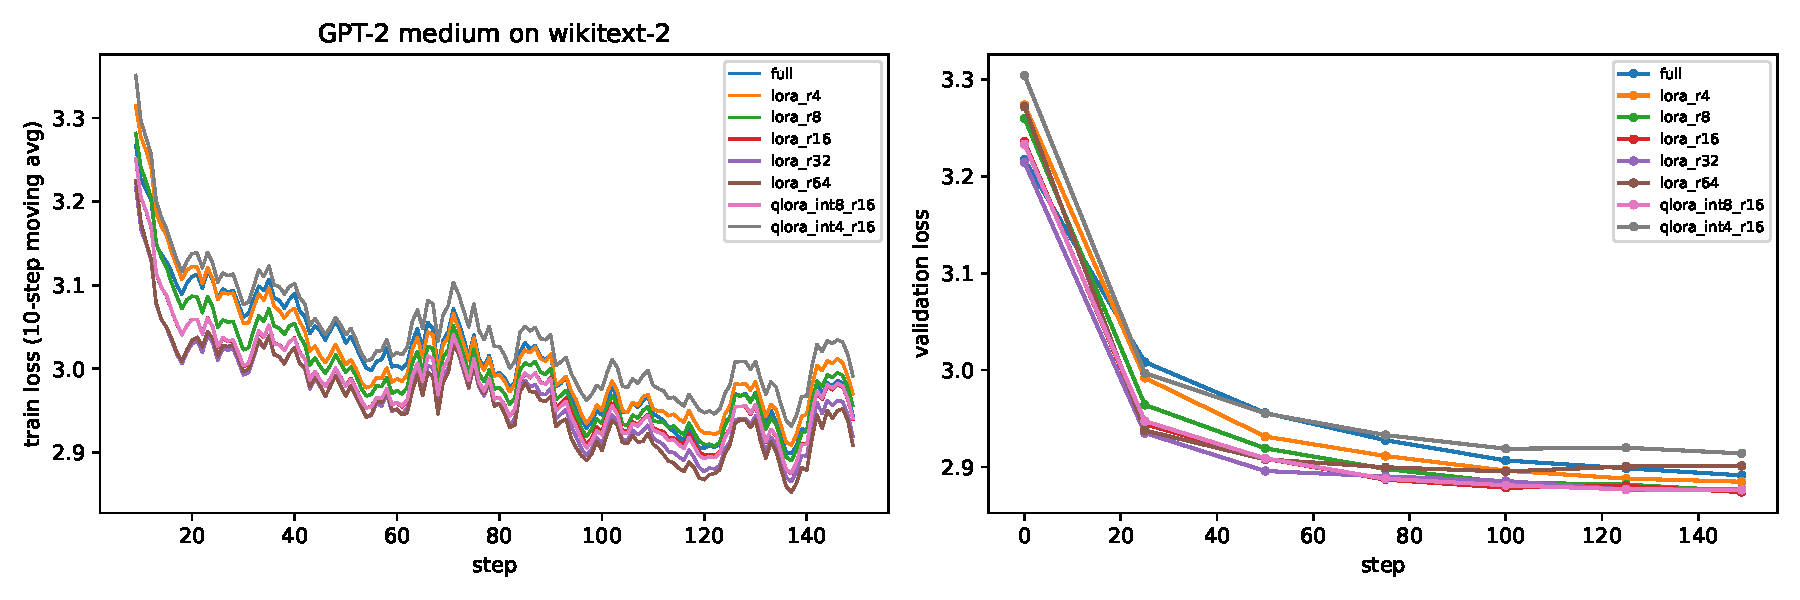
\includegraphics[width=\linewidth]{gpu_lora_curves.pdf}
\caption{训练损失（10 步滑动平均）与验证损失（每 25 步）。各 LoRA 配置和全量微调的曲线几乎重合。}
\label{fig:lora-curves}
\end{figure}

\begin{figure}[H]
\centering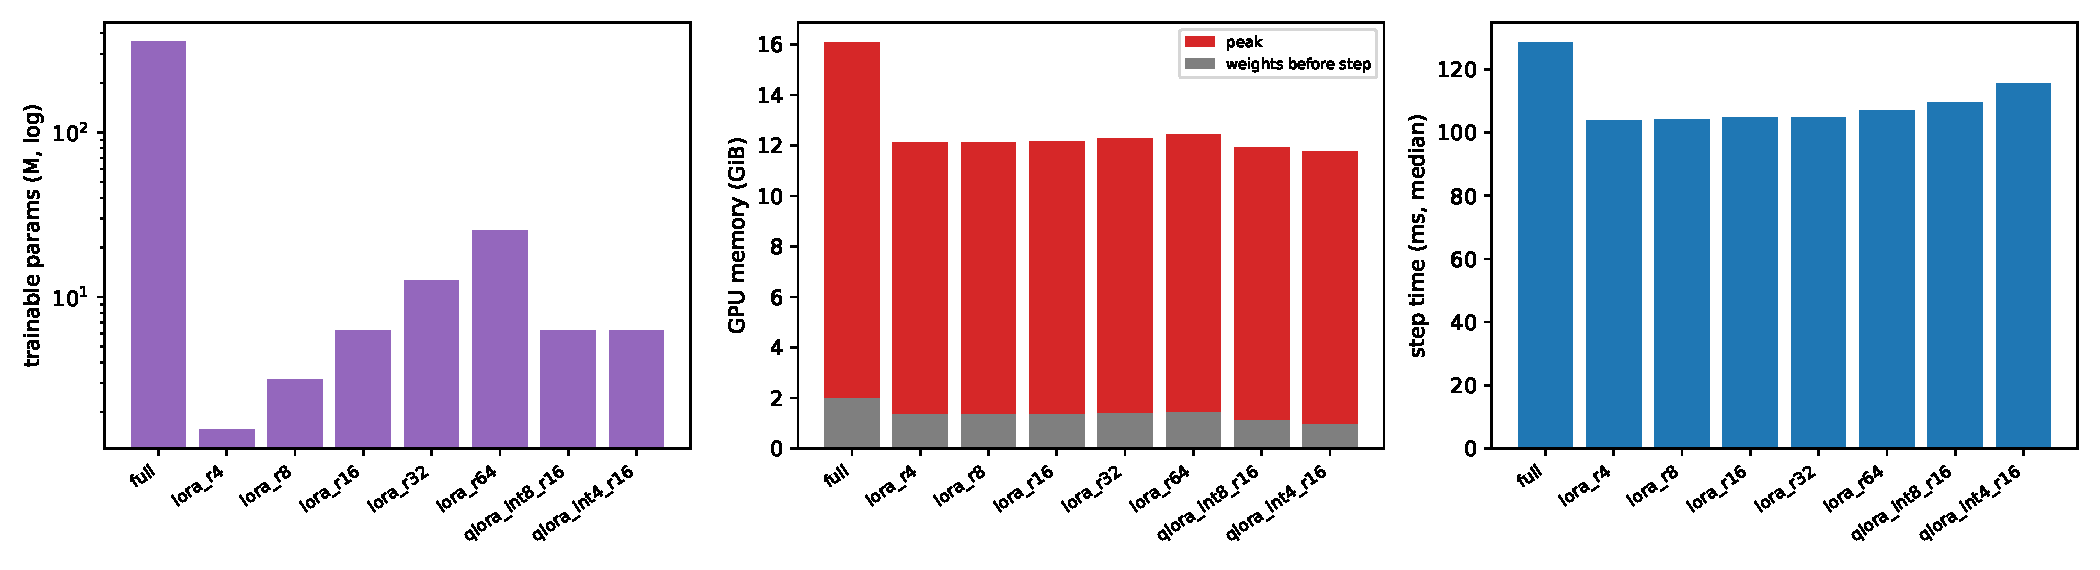
\includegraphics[width=\linewidth]{gpu_lora_cost.pdf}
\caption{可训参数（对数）、峰值/步前显存与步时。LoRA 各配置的可训参数相差十几倍，峰值显存却几乎不动，这就是“激活主导”的直观样子。}
\label{fig:lora-cost}
\end{figure}

\subsection{Q3 扩展：换到 7B——Qwen2.5-7B 上的同一套量化（RTX 6000D）}\label{sec:qwen7b}

GPT-2 的激活离群远弱于 6.7B 以上的模型，所以前面的量化结论可能对大模型不成立。为了检验这一点，我们把同一份 \texttt{gpu/quant\_llm.py} 原样跑在 Qwen2.5-7B 上：
bf16 载入，wikitext-2 test 共 29.9 万 token，校准用 128 × 1024 token，评估按 HF ctx 1024 的协议。原始结果在 \nolinkurl{artifacts/raw/rtx6000d/quant_ppl_Qwen2.5-7B.jsonl}。

\begin{figure}[H]
\centering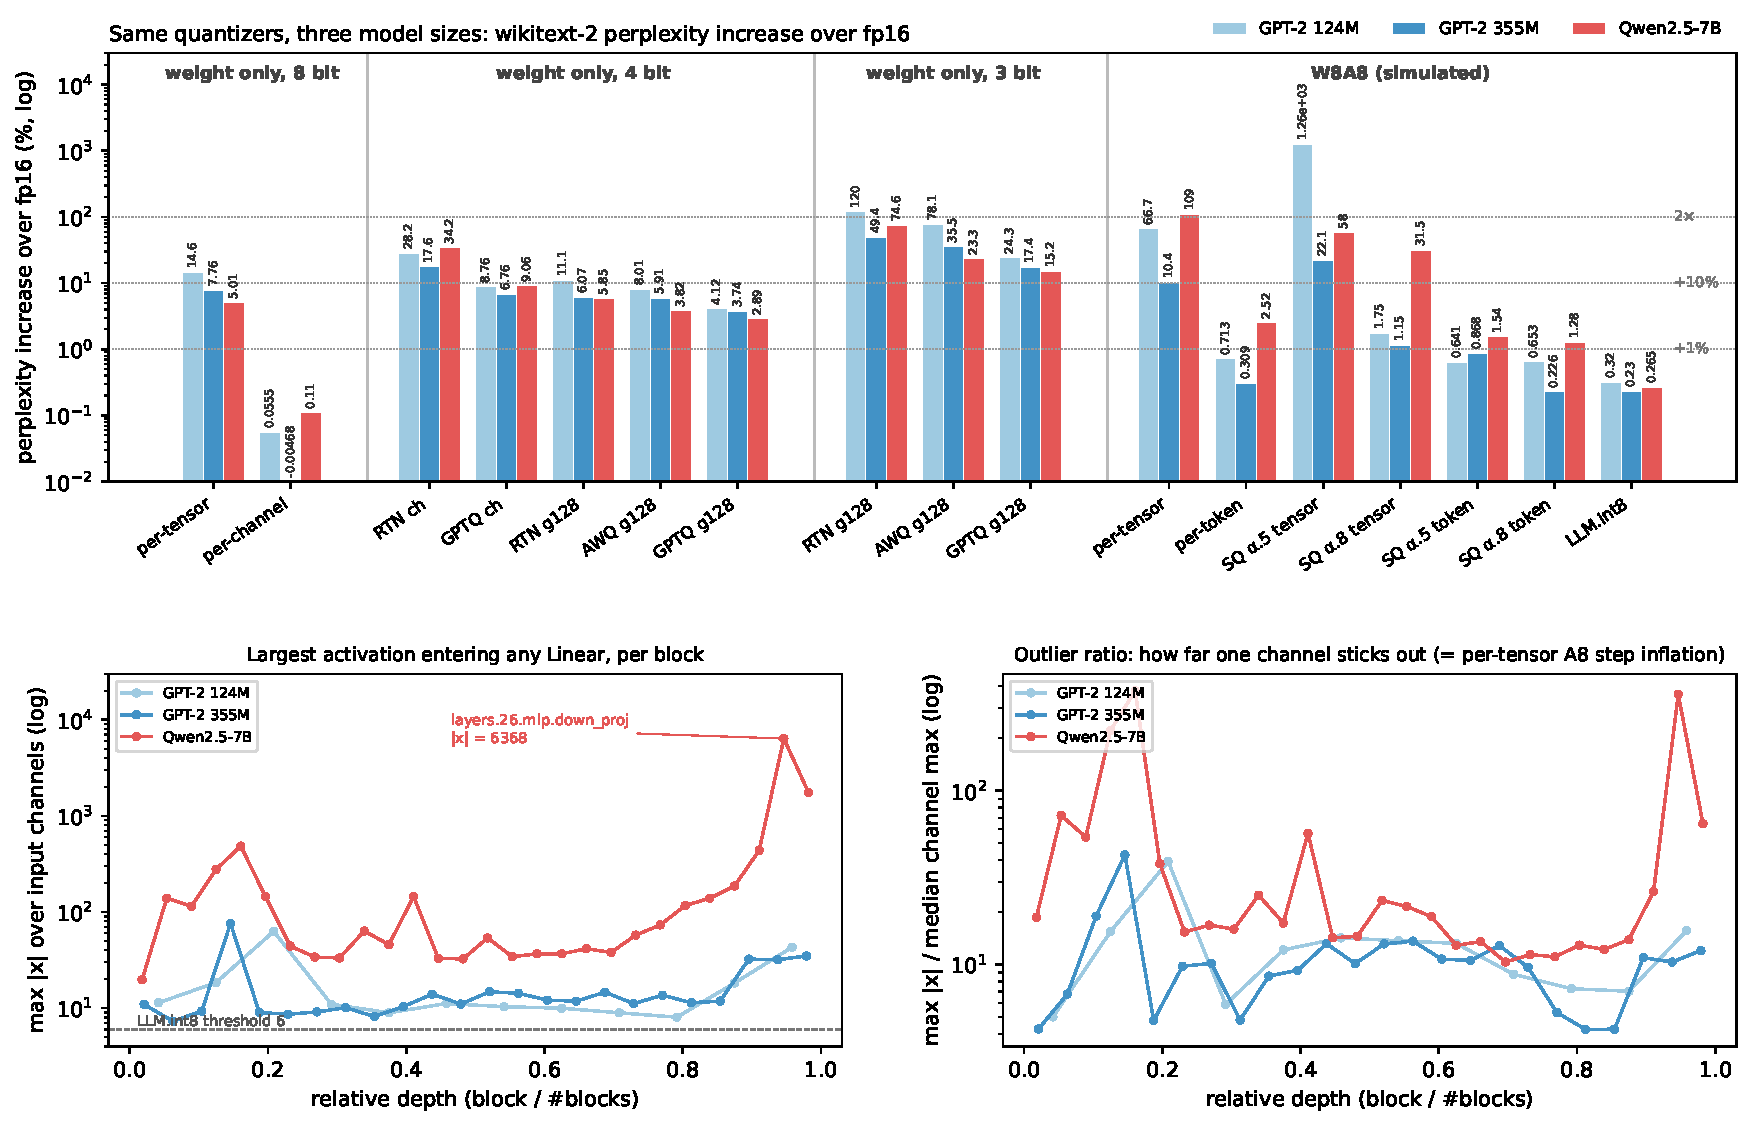
\includegraphics[width=\linewidth]{gpu_quant_scale.pdf}
\caption{三个规模上各方法相对 fp16 的困惑度增量，以及 Qwen2.5-7B 各层 Linear 输入的通道最大值（第 26 层 \texttt{down\_proj} 有 |x| = 6368 的离群）。}
\label{fig:qwen7b}
\end{figure}

\Cref{tab:qwen7b} 把三个模型放在一起，统一用相对 fp16 的增量表示，这样不同规模之间可以直接比较。

\begin{table}[H]
\centering\small
\caption{相对 fp16 的困惑度增量（Qwen2.5-7B fp16 为 7.639）}\label{tab:qwen7b}
\begin{tabular}{lrrr}
\toprule
方法 & GPT-2 124M & GPT-2 355M & Qwen2.5-7B \\
\midrule
W8 逐张量 / 逐通道 & +14.6\% / +0.06\% & +7.8\% / −0.005\% & +5.0\% / +0.11\% \\
W4 g128：RTN / AWQ / GPTQ & +11.1 / +8.0 / +4.1\% & +6.1 / +5.9 / +3.7\% & +5.9 / +3.8 / +2.9\% \\
W3 g128：RTN / AWQ / GPTQ & +120 / +78 / +24\% & +49 / +36 / +17\% & +75 / +23 / +15\% \\
W4 逐通道：RTN / GPTQ & +28 / +8.8\% & +18 / +6.8\% & +34 / +9.1\% \\
W8A8 逐张量 / 逐 token & +67 / +0.71\% & +10 / +0.31\% & \textbf{+109} / +2.5\% \\
SmoothQuant α=0.5 / 0.8（逐张量） & +1260 / +1.8\% & +22 / +1.2\% & +58 / +32\% \\
SmoothQuant α=0.5 / 0.8（逐 token） & +0.64 / +0.65\% & +0.87 / +0.23\% & +1.5 / +1.3\% \\
LLM.int8（阈值 6） & +0.32\% & +0.23\% & \textbf{+0.27\%} \\
\bottomrule
\end{tabular}
\end{table}

\begin{findingbox}[：权重量化随规模变容易，激活量化随规模变难]
W4 g128 GPTQ 从 +4.1\% 降到 +2.9\%，W3 GPTQ 从 +24\% 降到 +15\%；W8A8 逐张量却从 GPT-2 355M 的 +10\% 涨到 7B 的 +109\%。
\end{findingbox}

激活量化变难的原因可以在 \cref{fig:qwen7b} 右侧直接看到。Qwen 第 26 层 \texttt{mlp.down\_proj} 的输入里有一个通道 |x| = 6368，是该层通道最大值中位数的 358 倍。
逐张量量化的步长由这个通道决定，其余通道只剩下几个量化级。
SmoothQuant 逐张量在 α=0.8 时仍有 +32\%：离群太大，平滑把难度挪给权重之后，权重也装不下了；改用逐 token 激活再加平滑，才回到 +1.3\%。
LLM.int8 把 |x| > 6 的列留在 fp16，+0.27\% 是所有 W8A8 方法里最好的，代价是平均 700 列、最多 18702 列要走 fp16。

7B 上方法之间的差距也被拉开了：W3 g128 时 RTN +75\%、AWQ +23\%、GPTQ +15\%。AWQ 靠按激活幅度缩放通道起作用，所以在离群明显的模型上才有东西可缩。

这次实验里还踩到一个坑。GPTQ 第一次运行时在 \texttt{down\_proj}（输入有 18944 维）上报 Cholesky 非正定：离群通道把加了 1\% 阻尼的 fp32 Hessian 的条件数撑得太大。
现在 \texttt{gptq\_quantize} 改用 float64 做分解，失败时把阻尼放大 10 倍、100 倍重试；三个 GPTQ 配置各用了 967 s。

\begin{caveatbox}
困惑度协议（HF ctx 1024）与 edge-deploy llama-cpp-7b 的 llama-perplexity ctx 512 不同，两边数字不能直接比；W8A8 全部是精度模拟（fp16 GEMM），不含速度；
只有一个 7B 模型，离群通道的位置与幅度是 Qwen2.5 的特性。
\end{caveatbox}

\section{与理论模型的对照}

前面的实测反复用到几个简单的模型：时间等于字节除以带宽、tile 的强度、GEMV 的字节下限。这一节把它们推一遍，说明实测数字是怎么从这些公式里来的。

\subsection{融合：时间 = 字节 / 带宽}

设一条逐元素或行归约链在 eager 下有 $k$ 个 kernel，第 $i$ 个读 $r_i$、写 $w_i$ 个字节。eager 的总流量和融合后的下界分别为
\begin{equation}
B_{\text{eager}}=\sum_{i=1}^{k}(r_i+w_i),\qquad B_{\text{fused}}=\sum_{\text{图输入}}|x|+\sum_{\text{图输出}}|y| .
\label{eq:fusion-bytes}
\end{equation}
访存受限时 $T\approx B/\beta$，所以融合加速的上界就是 $B_{\text{eager}}/B_{\text{fused}}$。

以 RMSNorm 为例，设 bf16 输入 $x$ 占 $S$ 字节，逐步数一下。先上转 fp32（读 $S$ 写 $2S$），再平方（读 $2S$ 写 $2S$），按行求均值（读 $2S$），
乘 rstd（读 $2S$ 写 $2S$），乘权重（读 $2S$ 写 $2S$），最后下转 bf16（读 $2S$ 写 $S$）。合计约 $20S$ 量级，而融合只需要 $2S$。
dispatch 计数器给出 2685 MB / 268 MB = 10.0$\times$，实测是 9.86$\times$（\cref{tab:fusion}）。
如果 $\beta$ 取实测的 1.53 TB/s，$M{=}16384$ 时理想的 268 MB 需要 175 µs，与 Inductor 的 174.9 µs 吻合到 0.1\%。

\paragraph{为什么 MLP 的融合收益小。}MLP 的 FLOPs 为 $2\cdot T\cdot d\cdot 4d\cdot 2 = 16Td^2$。$T{=}4096,d{=}1024$ 时是 68.7 GFLOP，按 209.5 TFLOP/s 需要 328 µs。
能被融合省掉的，是 LN 输出、$[T,4d]$ 的 GELU 输入与输出，以及 $[T,d]$ 的残差前张量的写和读。实验室模型给出流量从 293.6 MB 降到 125.8 MB，省 167.8 MB，按 1.79 TB/s 约 94 µs。
所以全融合的上界大致是 $(328+\text{剩余访存})$ 相对 $(328+94+\dots)$，也就是 $\le 20\%$；实测 max-autotune 拿到了 15\%。

GEMM 和逐元素算子为什么落在 roofline 的两边，可以用 RTX 5090 的脊点来判断：
\begin{equation}
I^{*}=\frac{P}{\beta}=\frac{209.5\times10^{12}}{1.792\times10^{12}}\approx 117\ \text{FLOP/B},
\end{equation}
$[T,d]\times[d,4d]$ 的 GEMM 强度约为 $\frac{2\cdot T\cdot d\cdot 4d}{2(Td+4d^2+4Td)}$，$T{=}4096,d{=}1024$ 时约 683 FLOP/B，远大于 $I^*$，是计算受限的；逐元素算子的强度不到 1 FLOP/B，是访存受限的。

\subsection{GEMM 分块：强度、共享内存与波次}

Q2 里的三个现象（小 tile 在方阵上反而最好、一些配置跑不起来、瘦长形状偏好小 tile）分别对应三个约束。
第一个是强度。一个 $B_M\times B_N$ 的 C 块沿 K 每走一步，读 $(B_M+B_N)B_K$ 个元素、做 $2B_MB_NB_K$ 次运算，片上强度为
\begin{equation}
I_{\text{tile}}=\frac{2B_MB_NB_K}{2(B_M+B_N)B_K}=\frac{B_MB_N}{B_M+B_N}\ \text{FLOP/B (fp16)}.
\end{equation}
64$\times$64 只有 32 FLOP/B，低于 DRAM 的脊点 117，却是 $4096^3$ 上的最优。原因是 $4096^3$ 的 A、B 各 32 MB，都在 96 MB 的 L2 里，真正起作用的是 L2 带宽（数 TB/s 量级），脊点降到约 30--40 FLOP/B。
只按 DRAM 带宽建模的波次 roofline 因此偏爱大 tile，排错了顺序。

第二个是共享内存。Triton 的软件流水线要保留 $s-1$ 份缓冲：
\begin{equation}
(s-1)\cdot(B_M+B_N)\cdot B_K\cdot 2\ \text{B} \le 101376\ \text{B},
\end{equation}
例如 $32\times256\times64$、$s{=}4$ 需要 $3\cdot288\cdot64\cdot2 = 110592$ B，正是报错信息里的数字。

第三个是波次，即 $\lceil \#\text{tiles}/170\rceil$。$M{=}256$ 时用 128$\times$256 只有 32 个 tile，利用率 $32/170=19\%$。

\subsection{weight-only 量化：batch 1 下时间 $\propto$ 权重字节}

batch-1 GEMV 的 FLOPs 为 $2NK$，字节为 $NK\cdot b/8$（$b$ 为权重位宽），所以强度是 $16/b$ FLOP/B，bf16 为 1，int4 为 4，都远低于 117。于是时间只由字节决定：
\begin{equation}
T_{\text{GEMV}}\approx\frac{NK\,b/8+\text{scale 字节}}{\beta},\qquad \text{加速}_{\text{W4 vs bf16}}\le\frac{16}{4+16/g}=3.76\ (g=128).
\label{eq:w4bound}
\end{equation}
这也解释了 decode 与 prefill 上 W8A8 与 W4A16 之争。decode 是 GEMV，W4A16 读的字节少一半；prefill 是大 GEMM，W8A8 能用 int8 tensor core 拿到更高的峰值。

\subsection{GPTQ 与 SmoothQuant 的公式}

GPTQ 最小化的是层输出误差，而不是权重误差：$\|WX-\hat WX\|_F^2=\operatorname{tr}(\Delta W H\Delta W^\top)$，其中 $H=XX^\top$。
量化第 $q$ 列之后，它用 OBS 的闭式更新把误差推给还没量化的列：
\begin{equation}
\delta_{:,F}=-\frac{w_{:,q}-\operatorname{quant}(w_{:,q})}{[H^{-1}]_{qq}}\,[H^{-1}]_{q,F}.
\end{equation}
用 $H^{-1}$ 的上三角 Cholesky 因子，可以按列顺序一次算出所有的 $[H^{-1}]_{q,F}$，这是 GPTQ 相对 OBQ 能做到 $O(d^3)$ 的原因。
SmoothQuant 依据的是恒等式 $XW^\top=(X\operatorname{diag}(s)^{-1})(W\operatorname{diag}(s))^\top$，把激活的通道尺度挪给权重，$s_j=\max|X_j|^\alpha/\max|W_j|^{1-\alpha}$。这个恒等式在测试 \path{test_smoothquant_identity_without_quant_noise} 中验证过。

\subsection{LoRA/QLoRA 的显存账}

AdamW 全量微调每个参数要 16 B：fp32 权重 4 B、梯度 4 B、两个矩 8 B。GPT-2 medium 有 354.8M 参数，静态状态就是 5.68 GB。
LoRA 冻结的基座只需要 bf16 权重，每参数 2 B（0.71 GB）；换成 int8 是 1 B，int4 约 0.53 B（含 g128 的 scale）。可训参数为 $r\cdot\sum_\ell(d_{\text{in}}+d_{\text{out}})$。
但峰值显存里还有激活。batch $8\times512$、词表 50257 时，fp32 logits 一份就是 $8\cdot512\cdot50257\cdot4=0.82$ GB，而前向、softmax 和反向都要各存一份。

\section{面试专题}

\subsection{20 秒结论}

\begin{quote}
在 RTX 5090 上，访存受限链的 \texttt{torch.compile} 加速正好等于 eager 与融合的字节比：RMSNorm 的字节比是 10.0$\times$，实测 9.86$\times$，融合后 1.53 TB/s，已经顶到带宽墙。
含 GEMM 的 MLP 只快 15\%，而且要开 max-autotune，付出 11.7 倍的编译时间。
量化方面，int8 per-channel 无损；int3 时 GPTQ 把 GPT-2 的困惑度从 65.9 拉回 37.2。
batch 1 下 W8/W4 GEMV 分别快 1.8--2.0$\times$ 和 2.3--2.7$\times$，原因只是少读字节，前提是反量化融合进 kernel，否则会慢 10--23$\times$。
\end{quote}

\subsection{STAR 故事}

S（情境）：我想验证“图层融合能省多少时间”。CPU 上的模型预测，MLP 的流量降 49\%，时间却只降 16\%。

T（任务）：在真实 GPU 上测出 eager 与 Inductor 的字节、kernel 数和时间，判断这个模型可不可信，以及 max-autotune 值不值得默认打开。

A（行动）：我写了一个 \texttt{TorchDispatchMode} 字节计数器来统计 eager 搬的字节，用 profiler 数 kernel，在 5 条访存受限链 $\times$ 4 个尺寸 $\times$ 4 种模式上做了测量，并把实验室图 IR 换成 5090 的参数直接预测 MLP。

R（结果）：访存受限链的实测加速与字节比相差 $<$7\%；实验室模型预测 MLP 不融合 435.7 µs（实测 419.4），全融合 338.1 µs（实测 356.8）。
过程中还发现 max-autotune 的 CUDA graph 要拷贝输入，让 128 MB 级的访存受限 kernel 慢了 2.08$\times$（364.0 vs 174.9 µs）。
所以我的结论是：serving 的 decode 路径开 CUDA graph，prefill 和训练这类大张量路径用 \texttt{max-autotune-no-cudagraphs}。

\subsection{追问}

\begin{iqbox}{torch.compile 为什么能让 RMSNorm 快 10 倍，却让 MLP 几乎不变？}
因为融合省的是中间张量的读写，而 RMSNorm 几乎全是这种读写，MLP 的时间却几乎都在 GEMM 里。
RMSNorm 在 eager 下有 9 个 kernel，每一步都把 fp32 中间张量写回显存再读出来，共 2685 MB；融合后只读 $x$、写 $y$，268 MB。访存受限时时间正比于字节，所以快了 9.86$\times$。
MLP 有 83\% 以上的时间在两个计算受限的 GEMM 里，cuBLAS 又已经做了 bias epilogue，能融合的只剩 GELU 和残差约 168 MB 的往返，上界约 20\%；实测 default 快 1.2\%，max-autotune 快 15\%。

常见的错答是“compile 生成了更好的 kernel，所以什么都会变快”。实际上它默认对 GEMM 仍然调用 cuBLAS，收益只来自删掉中间张量。
\end{iqbox}

\begin{iqbox}{max-autotune 一定比 default 快吗？}
不一定，大张量上它可能慢一倍。它会打开 CUDA graph（cudagraph trees），而输入不在静态地址时，每次 replay 前都要拷贝输入。
对 $16384\times4096$ 的 softmax，default 是 175.3 µs，max-autotune 是 363.4 µs，关掉 CUDA graph 的 no-cudagraphs 是 175.2 µs。
它还要 benchmark GEMM 模板，MLP 编译 6.9 s、block 12.9 s；很多为 H100 设计的模板需要 128--144 KB 共享内存，在 sm\_120 的 99 KB 上直接失败。

常见的错答是“max-autotune 只是多试几个配置，最差也和 default 一样”。
\end{iqbox}

\begin{iqbox}{动态 shape 下 torch.compile 怎么避免反复重编译？}
把会变的维度标成动态，让它编一个符号形状图。默认的 automatic dynamic 第一次按静态 shape 编译，看到同一维度变化后再编一个符号形状图（我们 10 个长度共 2 个图、0.99 s）；
\texttt{mark\_dynamic} 一开始就编符号图（1 个图、0.54 s）；\texttt{dynamic=False} 每个新长度都重编（8 个图后到达 \texttt{cache\_size\_limit}，4.46 s）。
对 GEMM 主导的 MLP，符号形状图稳态没有损失：4096 token 时 420.2 vs 419.8 µs。

常见的错答是“dynamic shape 一定慢，所以应该全静态”。代价在编译和 guard，不在 kernel。
\end{iqbox}

\begin{iqbox}{Triton matmul 的 tile 怎么选？代价模型靠得住吗？}
tile 要同时满足强度、共享内存、SM 占用和寄存器四个约束，最优解随形状变化，解析模型靠不住，最终要实测。
片上强度 $B_MB_N/(B_M+B_N)$ 够用即可，A/B 在 L2 里时脊点更低；共享内存要满足 $(s-1)(B_M+B_N)B_K\cdot2\le99$ KB；C 块数要对得上 170 个 SM 的波次；
寄存器也是硬约束，256$\times$256 的 fp32 累加器要 256 KB。实测最优在 $4096^3$ 是 64$\times$64，$8192^3$ 是 128$\times$128，$M{=}256$ 是 128$\times$64。
复用型解析模型的 $\rho$ 为 0.65/0.36/0.10，波次模型为 0.26/0.21/0.72，各只看见一种效应，所以 Ansor 用学习型模型加实测。

常见的错答是“tile 越大复用越高，所以越快”。256$\times$256 在三个形状上都最差（75/78/14 TFLOP/s）。
\end{iqbox}

\begin{iqbox}{GPTQ 比 RTN 好在哪？什么时候没用？}
GPTQ 优化的是层输出误差，靠的是输入之间的相关性；输入不相关时它就没用。
它最小化 $\operatorname{tr}(\Delta WH\Delta W^\top)$，每量化一列就用 $H^{-1}$ 把误差补偿到还没量化的列上。int3 g128 时，GPT-2 124M 的困惑度从 RTN 的 65.92 降到 GPTQ 的 37.24。
但在 CPU 实验里，输入各向同性（$H\approx cI$）时，GPTQ 的测试误差是 28.2\%，反而比 RTN 的 26.4\% 差，因为补偿只拟合了校准噪声。

常见的错答是“GPTQ 让量化后的权重更接近原权重”。其实它的权重误差更大（CPU 实验中 0.28--0.39 vs 0.26），它优化的是输出。
\end{iqbox}

\begin{iqbox}{W4A16 和 W8A8 选哪个？}
看场景：decode 选 W4A16，因为它少读字节；prefill 选 W8A8，因为它能用更快的 int8 tensor core。
decode（batch 1 到小 batch）是 GEMV，强度 $16/b$ FLOP/B 远低于脊点 117，时间正比于权重字节：W4A16 在 $16384\times8192$ 上 62.2 µs，bf16 是 163.0 µs（2.62$\times$）。
prefill 是大 GEMM，计算受限：$M{=}8192$ 时 int8 679.4 TOP/s，bf16 226.9（3.0$\times$，因为 GeForce 上 bf16 的 fp32 累加是半速）。

常见的错答是“int4 比 int8 少一半位，所以永远快一倍”。W4 的解包开销让我们的 kernel 只到 0.98--1.11 TB/s，而且 prefill 时 W4A16 仍然要用 bf16 tensor core 计算。
\end{iqbox}

\begin{iqbox}{SmoothQuant 的 $\alpha$ 怎么选？}
在校准集上扫，因为它是模型相关的超参数，没有通用值。$\alpha$ 决定把多少激活的量化难度迁移到权重上。
GPT-2 124M 上，$\alpha{=}0.5$ 加 per-tensor 激活得到困惑度 407.25，比不平滑的 49.94 还差；$\alpha{=}0.8$ 得到 30.49。
如果激活能做 per-token 量化，W8A8 本身已经接近无损（30.18）。

常见的错答是“论文用 0.5，所以 0.5 是通用最优”。
\end{iqbox}

\begin{iqbox}{为什么非结构化剪枝在 GPU 上难以变快，2:4 呢？}
非结构化稀疏打乱了 tensor core 需要的稠密 tile，只能走 CSR 的间接寻址；2:4 是硬件认识的结构，但也要问题足够大才划算。
CSR 在 $4096^2$、$M{=}512$、50\% 稀疏时慢 18.5$\times$，到 99\% 稀疏才快 2.18$\times$。
2:4 每 4 个元素留 2 个，用 2 bit 元数据记录位置，稀疏 tensor core 直接跳过一半乘加，大 GEMM 上实测快 1.54--1.58$\times$；但 cuSPARSELt 在 sm\_120 上每次调用约有 445 µs 的开销，所以 $M\le2048$ 时更慢。
精度上，同为 50\%，幅值 2:4 让 GPT-2 的困惑度变成 735.95，Wanda 2:4 是 116.38。

常见的错答是“剪掉 50\% 权重就省 50\% 时间”。要省时间，需要硬件支持的结构和足够大的 $M$，精度损失还要靠激活感知的打分或再训练补回来。
\end{iqbox}

\begin{iqbox}{LoRA 省的显存到底在哪？QLoRA 又省在哪？}
LoRA 省的是优化器状态和梯度，QLoRA 再省冻结基座的权重；激活两者都不省。
全量 AdamW 每参数 16 B，GPT-2 medium 的 fp32 梯度加两个矩约 3.97 GiB，正好是全量（16.07 GiB）与 LoRA（12.10--12.45 GiB）峰值之差；剩下的 10.7 GiB 是激活。
QLoRA 把冻结基座从每参数 2 B 压到约 0.5 B，对 355M 只省 0.41 GiB，对 65B 模型却是 130 GB 变成约 35 GB，决定了能不能放进单卡。
实现上要注意：反量化出的权重如果交给 \texttt{F.linear}，autograd 会把它存进计算图，显存一点不省；要用自定义 \texttt{autograd.Function}，只存量化张量，反向时重算。

常见的错答是“LoRA 可训参数只有 0.9\%，所以显存也只要 1\%”。激活和基座权重都还在。
\end{iqbox}

\begin{iqbox}{如何测一个“访存受限”kernel 的真实带宽而不被 L2 骗？}
让工作集大于 L2（RTX 5090 是 96 MB），或者轮换多份副本。
我们的 LayerNorm 在 $4096\times4096$（67 MB）时 eager 显示 3.32 TB/s，高于 1.79 TB/s 的 GDDR7 峰值，这就是 L2 命中；GEMV 的 cold 模式在 $11008\times4096$ W8 上把“带宽”从 hot 的 2.67 TB/s 拉回 1.57 TB/s。

常见的错答是“超过峰值说明计时有 bug”。这是缓存层次造成的，不是 bug。
\end{iqbox}

\begin{caveatbox}
\begin{itemize}
\item W8A8、SmoothQuant、LLM.int8 都是“量化-反量化”的精度模拟，用 fp16 GEMM 计算，没有测这些方案真实的 int8 端到端速度；速度只在单个 GEMM/GEMV 上测过。
\item 困惑度只在 GPT-2 124M/355M 上测；它们的激活离群远弱于 6.7B 以上的模型，LLM.int8/SmoothQuant 的必要性在大模型上会更突出。不能把“per-token W8A8 近无损”外推到 LLaMA/OPT 大模型。
\item AWQ 是简化版（只在 $\overline{|x|}^a$ 上网格搜索，用代理误差选 $a$，没有 clip 搜索），GPTQ 没有 act-order；两者的排名不代表原论文实现的排名。
\item 低精度 GEMM 的 $N{=}K{=}4096$ 权重（32 MB）常驻 L2，小 $M$ 的吞吐偏乐观；GEMV 区分了 hot/cold，GEMM 没有。
\item 融合实验的“理想字节”是下界；Inductor 的真实 DRAM 流量没有用 Nsight Compute 测量，带宽数字是“理想字节 / 时间”。小尺寸的数字被 Python/guard 开销（11--27 µs）主导。
\item Triton matmul 网格只覆盖 4 个超参维度，GROUP\_M 固定为 8，没有试 persistent/TMA/warp-specialized kernel；“超过 cuBLAS”只在 fp16 方阵上成立，瘦长形状上 cuBLAS 仍快 6\%。
\item 编译时间受服务器只给 2 个 CPU 核的影响，绝对值偏大；但模式之间的比例可信。
\item 剪枝只做了一次性剪枝、没有再训练；2:4 的 445 µs 调用下限可能是 PyTorch 2.8 的 cuSPARSELt 路径在 sm\_120 上的实现问题，不应当作硬件特性。
\item LoRA 只训练了 150 步、单个随机种子；loss 相差 0.01 量级在噪声范围内，“LoRA 略好于全量”不能推广，能下的结论只有“在这个预算下不比全量差”。
\item RTX 5090 的峰值取的是规格值；实测 GEMM（fp16 221.5 TFLOP/s、int8 679.4 TOP/s）说明卡的实际频率高于标称 boost，文中的百分比应按实测上界来理解。
\end{itemize}
\end{caveatbox}

\section{结论}

读完这份报告，值得带走的是下面六点。

\begin{enumerate}
\item 融合的收益可以先算再测。访存受限时加速 $\approx B_{\text{eager}}/B_{\text{fused}}$，实测吻合到 7\% 以内；计算受限时，上界由“可删的中间张量字节 / 总时间”决定，MLP 只有 15--20\%。实验室的 CPU 图 IR 换上 RTX 5090 参数后，对 MLP 的预测误差为 $-3.7\%$/$+5.5\%$。
\item 编译器的工程代价是真实的。max-autotune 的编译时间是 default 的 11.7--22$\times$，CUDA graph 对大张量是负优化；动态 shape 应该 \texttt{mark\_dynamic}（1 个图 0.54 s，静态策略要 8 个图 4.46 s）。
\item 调度搜索离不开实测。解析代价模型的排序相关只有 0.10--0.72，而且不同模型在不同形状上失效；它们适合剪掉搜索空间里的坏配置（OOR、过小的 tile），最终选择要靠 benchmark（autotune）或学习型模型（Ansor）。
\item 量化要同时用对粒度和数据。per-channel 解决权重的重尾，int4 以下必须用数据（GPTQ 的 Hessian 补偿、AWQ 的激活缩放）；激活离群按通道出现，per-token 或 LLM.int8 的分解最稳，SmoothQuant 需要调 $\alpha$。
\item 速度只来自少读字节或更高的峰值。batch 1 下 weight-only 量化按字节比加速，但必须把反量化融合进 kernel；prefill 下 int8 tensor core 给出 3$\times$ 的峰值；2:4 在大 GEMM 上快 1.5$\times$，非结构化稀疏在 GPU 上要 $>$95\% 才划算。
\item LoRA 省的是优化器状态。355M 模型上峰值显存 $-25\%$、步时 $-19\%$，激活不变；QLoRA 的基座压缩要到数十 B 参数才起决定作用。
\end{enumerate}

\begin{thebibliography}{99}
\bibitem{tvm} T.~Chen et al. TVM: An Automated End-to-End Optimizing Compiler for Deep Learning. OSDI 2018.
\bibitem{ansor} L.~Zheng et al. Ansor: Generating High-Performance Tensor Programs for Deep Learning. OSDI 2020.
\bibitem{taso} Z.~Jia et al. TASO: Optimizing Deep Learning Computation with Automatic Generation of Graph Substitutions. SOSP 2019.
\bibitem{xla} XLA: Optimizing Compiler for Machine Learning. Google, 2017; and A.~Sabne, XLA: Compiling Machine Learning for Peak Performance, 2020.
\bibitem{pt2} J.~Ansel et al. PyTorch 2: Faster Machine Learning Through Dynamic Python Bytecode Transformation and Graph Compilation. ASPLOS 2024.
\bibitem{triton} P.~Tillet, H.~T.~Kung, D.~Cox. Triton: An Intermediate Language and Compiler for Tiled Neural Network Computations. MAPL 2019.
\bibitem{halide} J.~Ragan-Kelley et al. Halide: A Language and Compiler for Optimizing Parallelism, Locality, and Recomputation in Image Processing Pipelines. PLDI 2013.
\bibitem{llmint8} T.~Dettmers et al. LLM.int8(): 8-bit Matrix Multiplication for Transformers at Scale. NeurIPS 2022.
\bibitem{smoothquant} G.~Xiao et al. SmoothQuant: Accurate and Efficient Post-Training Quantization for Large Language Models. ICML 2023.
\bibitem{gptq} E.~Frantar et al. GPTQ: Accurate Post-Training Quantization for Generative Pre-trained Transformers. ICLR 2023.
\bibitem{obq} E.~Frantar, D.~Alistarh. Optimal Brain Compression: A Framework for Accurate Post-Training Quantization and Pruning. NeurIPS 2022.
\bibitem{awq} J.~Lin et al. AWQ: Activation-aware Weight Quantization for LLM Compression and Acceleration. MLSys 2024.
\bibitem{lora} E.~J.~Hu et al. LoRA: Low-Rank Adaptation of Large Language Models. ICLR 2022.
\bibitem{qlora} T.~Dettmers et al. QLoRA: Efficient Finetuning of Quantized LLMs. NeurIPS 2023.
\bibitem{deepcomp} S.~Han, H.~Mao, W.~J.~Dally. Deep Compression: Compressing Deep Neural Networks with Pruning, Trained Quantization and Huffman Coding. ICLR 2016.
\bibitem{nm} A.~Mishra et al. Accelerating Sparse Deep Neural Networks. arXiv:2104.08378, 2021.
\bibitem{wanda} M.~Sun et al. A Simple and Effective Pruning Approach for Large Language Models (Wanda). ICLR 2024.
\bibitem{roofline} S.~Williams, A.~Waterman, D.~Patterson. Roofline: An Insightful Visual Performance Model for Multicore Architectures. CACM 2009.
\bibitem{gpt2} A.~Radford et al. Language Models are Unsupervised Multitask Learners. OpenAI, 2019.
\bibitem{wikitext} S.~Merity et al. Pointer Sentinel Mixture Models. ICLR 2017.
\end{thebibliography}

\end{document}
